\documentclass[reprint, amsmath,amssymb,aps,pre]{revtex4-2}

\usepackage[pdfborder={0 0 0.5 [3 2]}, plainpages=false]{hyperref}%
\usepackage[left=1in,right=1in,top=1in,bottom=1in]{geometry}%

\usepackage{enumerate}
\usepackage{amsfonts}
\usepackage{amsthm}
\usepackage{bbm}
\usepackage[table,xcdraw]{xcolor}
\usepackage{mathtools}
\usepackage{cool}
\usepackage{graphicx,epsfig}

\usepackage{subcaption}
\captionsetup{font={small},skip=0.25\baselineskip}
\captionsetup{justification=raggedright}
\captionsetup[subfigure]{font={small}, skip=1pt, singlelinecheck=false}

\usepackage[capitalize,nameinlink]{cleveref}
% Per SIAM Style Manual, "section" should be lowercase
\crefname{section}{section}{sections}
\crefname{subsection}{subsection}{subsections}
\Crefname{section}{Section}{Sections}
\Crefname{subsection}{Subsection}{Subsections}

% Per SIAM Style Manual, "Figure" should be spelled out in references
\Crefname{figure}{Figure}{Figures}

% Per SIAM Style Manual, don't say equation in front on an equation.
\crefformat{equation}{\textup{#2(#1)#3}}
\crefrangeformat{equation}{\textup{#3(#1)#4--#5(#2)#6}}
\crefmultiformat{equation}{\textup{#2(#1)#3}}{ and \textup{#2(#1)#3}}
{, \textup{#2(#1)#3}}{, and \textup{#2(#1)#3}}
\crefrangemultiformat{equation}{\textup{#3(#1)#4--#5(#2)#6}}%
{ and \textup{#3(#1)#4--#5(#2)#6}}{, \textup{#3(#1)#4--#5(#2)#6}}{, and \textup{#3(#1)#4--#5(#2)#6}}

% But spell it out at the beginning of a sentence.
\Crefformat{equation}{#2Equation~\textup{(#1)}#3}
\Crefrangeformat{equation}{Equations~\textup{#3(#1)#4--#5(#2)#6}}
\Crefmultiformat{equation}{Equations~\textup{#2(#1)#3}}{ and \textup{#2(#1)#3}}
{, \textup{#2(#1)#3}}{, and \textup{#2(#1)#3}}
\Crefrangemultiformat{equation}{Equations~\textup{#3(#1)#4--#5(#2)#6}}%
{ and \textup{#3(#1)#4--#5(#2)#6}}{, \textup{#3(#1)#4--#5(#2)#6}}{, and \textup{#3(#1)#4--#5(#2)#6}}

% Make number non-italic in any environment.
\crefdefaultlabelformat{#2\textup{#1}#3}

\hypersetup{hidelinks}

\def\noi{\noindent}
\def\T{{\mathbb T}}
\def\R{{\mathbb R}}
\def\N{{\mathbb N}}
\def\C{{\mathbb C}}
\def\Z{{\mathbb Z}}
\def\P{{\mathbb P}}
\def\E{{\mathbb E}}
\def\Q{\mathbb{Q}}
\def\ind{{\mathbb I}}

\DeclareMathOperator{\spn}{span}
\DeclareMathOperator{\ran}{range}

\graphicspath{ {images/} }

\newtheorem{lemma}{Lemma}
\newtheorem{theorem}{Theorem}
\newtheorem{corollary}{Corollary}
\newtheorem{definition}{Definition}
\newtheorem{proposition}{Proposition}
\newtheorem{hypothesis}{Hypothesis}
\newtheorem{remark}{Remark}

\begin{document}

\section{Introduction}

\section{Mathematical Model}

We consider an implementation of the Aubry-Andr\'e model \cite{Aubry1980} of a linear array of coupled waveguides
\begin{equation}\label{eq:model}
i \frac{d u_n}{d z} + J_n(z) u_{n+1} + J_{n-1}(z)u_{n-1} + g|u_n|^2 u_n = 0,
\end{equation}
where $u_n(z)$ is the complex amplitude of the waveguide at site $n$ in the integer lattice, and $g$ quantifies the strength of the cubic nonlinearity. The sites in the lattice are coupled with their nearest neighbors via the $z$-dependent coupling functions $J_n(z)$. The coupling functions $J_n(z)$ are periodic in $z$ with spatial period $L$, which we will refer to as the coupling period. The choice of $J_n(z)$
\begin{equation}\label{eq:Jn}
J_n(z) = J_0 + C \cos^2\left( \frac{\pi}{L}z + \frac{4 \pi}{3} n + \frac{\pi}{6} \right)
\end{equation}
groups the lattice sites into unit cells comprising three waveguides each (\cref{fig:J}), since $J_n(z) = J_m(z)$ for $m \equiv n\,(\text{mod}\,3)$.

\begin{figure}
    \centering
    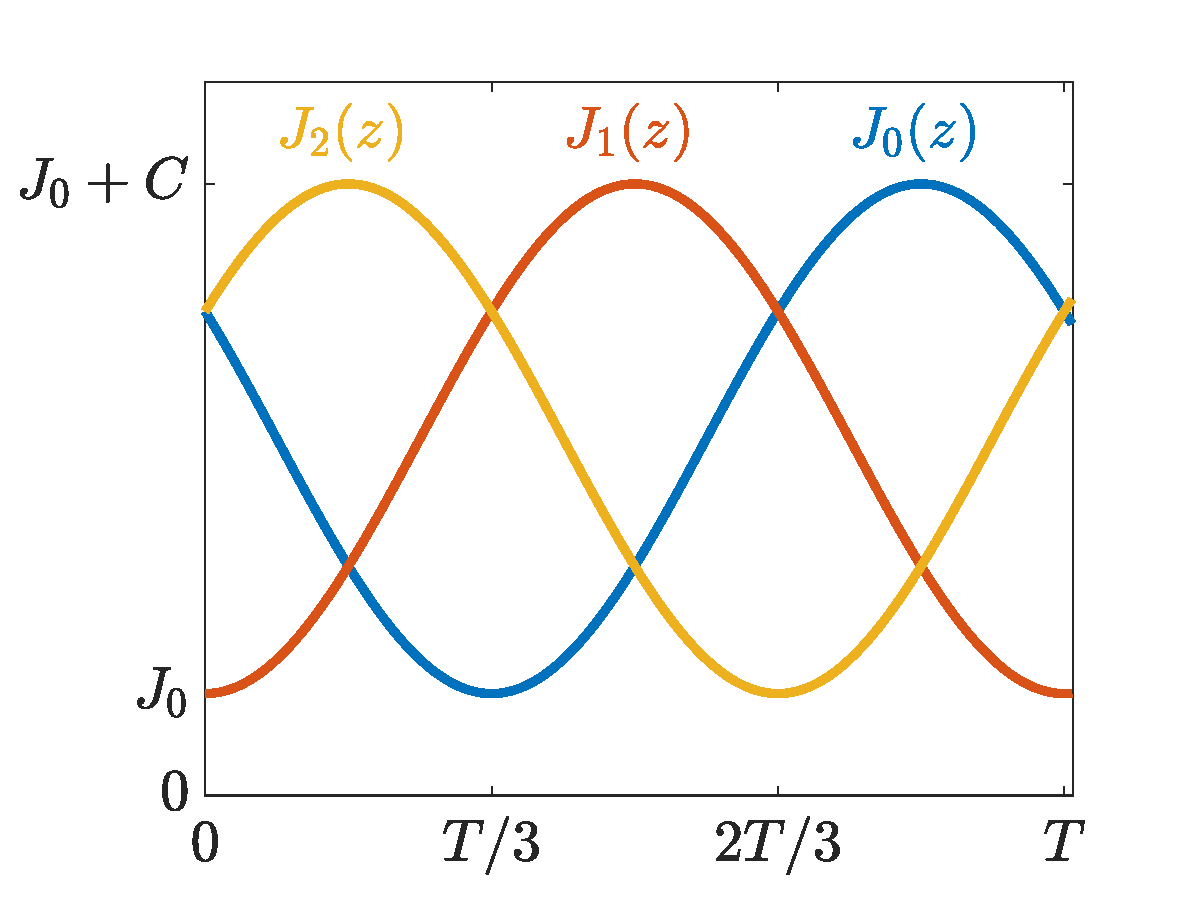
\includegraphics[width=8cm]{J.eps}
    \caption{Coupling functions $J_0(z)$, $J_1(z)$, and $J_2(z)$ of $z$-dependent nearest-neighbor couplings over one spatial period $L$.}
    \label{fig:J}
\end{figure}

When $C = 0$, the nearest neighbor coupling is constant, and equation \cref{eq:model} reduces to the discrete nonlinear Schr\"odinger equation \cref{eq:modelDNLS}, written in a co-rotating frame with frequency $2 J_0$.
\begin{equation}\label{eq:modelDNLS}
i \frac{d u_n}{d z} + J_0( u_{n+1} - 2 u_n + u_{n-1}) + g|u_n|^2 u_n + 2 J_0 u_n = 0,
\end{equation}
In order to use the spatial period $L$ as a parameter, we rescale the propagation distance using the change of variables $z = L Z$ so that the coupling period is always 1.
\begin{equation}\label{eq:modelZ}
\begin{aligned}
i \frac{1}{L} \frac{d u_n}{d Z} &+ J_n(Z) u_{n+1} + J_{n-1}(Z)u_{n-1} + g|u_n|^2 u_n = 0 \\
J_n(Z) &= J_0 + C \cos^2\left( \pi Z + \frac{4 \pi}{3} n + \frac{\pi}{6} \right)
\end{aligned}
\end{equation}
At any propagation distance $Z$, the power of the solution is the squared $\ell^2$ norm of the solution
\begin{equation}
P(u_n) = \sum_{n} | u_n(Z) |^2,
\end{equation} 
where the sum is taken over the entire lattice. The power is conserved, i.e. $P(u_n)$ is independent of $Z$. Using equation \cref{eq:modelZ} and its complex conjugate, we derive the Liouville-Von Neumann equation for the density matrix elements $\rho_{mn} = \overline{u_n} u_m$
\begin{equation}\label{eq:rhoeq}
\begin{aligned}
\frac{d}{dZ} \rho_{mn} &= iL \Big[ J_m(Z) \rho_{m+1,n} + J_{m-1}(Z) \rho_{m-1,n} \\
&\qquad -J_n(Z) \rho_{m,n+1} - J_{n-1}(Z) \rho_{m,n-1} \big] \\
&\qquad + iLg\left( \rho_{mm}^2 - \rho_{nn}^2 \right) \rho_{mn}
\end{aligned}
\end{equation}
The evolution of power of the solution at lattice site $n$, which is given by $\rho_{nn}^2 = | u_n |^2$, is
\begin{equation}\label{eq:powerevol}
\begin{aligned}
\frac{d}{dZ} \rho_{nn} &= iL \Big[ J_n(Z) \rho_{n+1,n} + J_{n-1}(Z) \rho_{n-1,n} \\
&\qquad -J_n(Z) \rho_{n,n+1} - J_{n-1}(Z) \rho_{n,n-1} \big] \\
&= -2L\,\text{Im}\Big[ J_n(Z) \rho_{n+1,n} + J_{n-1}(Z) \rho_{n-1,n} \Big],
\end{aligned}
\end{equation}
where we used the fact that $\rho_{n,m} = \overline{\rho_{m,n}}$.
Using the last line of \cref{eq:powerevol}, we define the leftward and rightward fluxes at each lattice site $n$ by
\begin{equation}
\begin{aligned}
Q_n^L(Z) &= -2L\,J_{n-1}(Z)\,\text{Im}\left(J_{n-1}(Z) \rho_{n-1,n} \right) \\
Q_n^R(Z) &= -2L\,J_{n-1}(Z)\,\text{Im}\left(J_n(Z) \rho_{n+1,n} \right) 
\end{aligned}
\end{equation}
where positive flux denotes flow of power into site $n$. Since the power of the solution is conserved, $Q_n^R(Z) = -Q_{n+1}^L(Z)$ and $Q_n^L(Z) = -Q_{n-1}^R(Z)$.

\section{Single site evolution}

As an initial experiment, we perform evolution experiments starting with a single excited site at $Z=0$. Unless otherwise specified, the parameters in the section are $g=1$, $L=2\pi$, $J_0 = 0.05$, and $C=0.4$, and the simulations are run on a finite lattice with $m=30$ lattice points, with periodic boundary conditions on the ends of the lattice. For a single-site initial condition of sufficiently high power (between $P=2.25$ and $P=2.5$ for initial intensity at $n=0$, and between $P=2.15$ and $P=2.25$ for initial intensity at $n=-1$), the power remains concentrated at a single site, and this appears to be stable as $Z$ evolves (see bottom panel of \cref{fig:timestep0} and \cref{fig:timestep0}). As the initial power is lowered, this single-site solution becomes unstable; in both cases, when stability is lost, intensity initially radiates to the right in the lattice before dissipating throughout the lattice (bottom left of \cref{fig:timestep0} and \cref{fig:timestep0}). For lower power (between $P=0.5$ and $P=1$), the initial intensity moves either to the left in the lattice (for excited site at $n=0$, see top of \cref{fig:timestep0}) or to the right (for excited site at $n=-1$, see top of \cref{fig:timestep1}) before dissipating. One explanation for this observation is as follows. For the first third of the period ($Z \in [0,1/3]$), the strongest coupling is between site $n=0$ and $n=-1$ via $J_{-1} = J_2$ (see \cref{eq:Jn} and \cref{fig:J}), so intensity can flow to the left from $n=0$ to $n=-1$, which occurs when the initial power is sufficiently low. For $Z \in [1/3,2/3]$, the strongest coupling is between $n=-1$ and $n=-2$, and for $Z \in [1/3,2/3]$, the strongest coupling is between $n=-2$ and $n=-3$, thus we expect the intensity to travel three sites to the left over one period. Similarly, for the rightward moving solution starting at $n=-1$, the rightward coupling is strongest for a rightward sequence of sites on the $Z$ intervals $[0,1/3]$, $[2/3,1]$, and $[4/3,5/3]$, thus this solution moves to the right three sites in two periods. A similar rightward moving behavior occurs when the initial excited site is $n=1$ (not shown). The first coupling for $n=1$ is to the right on the interval $[1/3, 2/3]$; the behavior is then similar to that of the rightward moving solution for $n=-1$. 

\begin{figure}
    \centering
    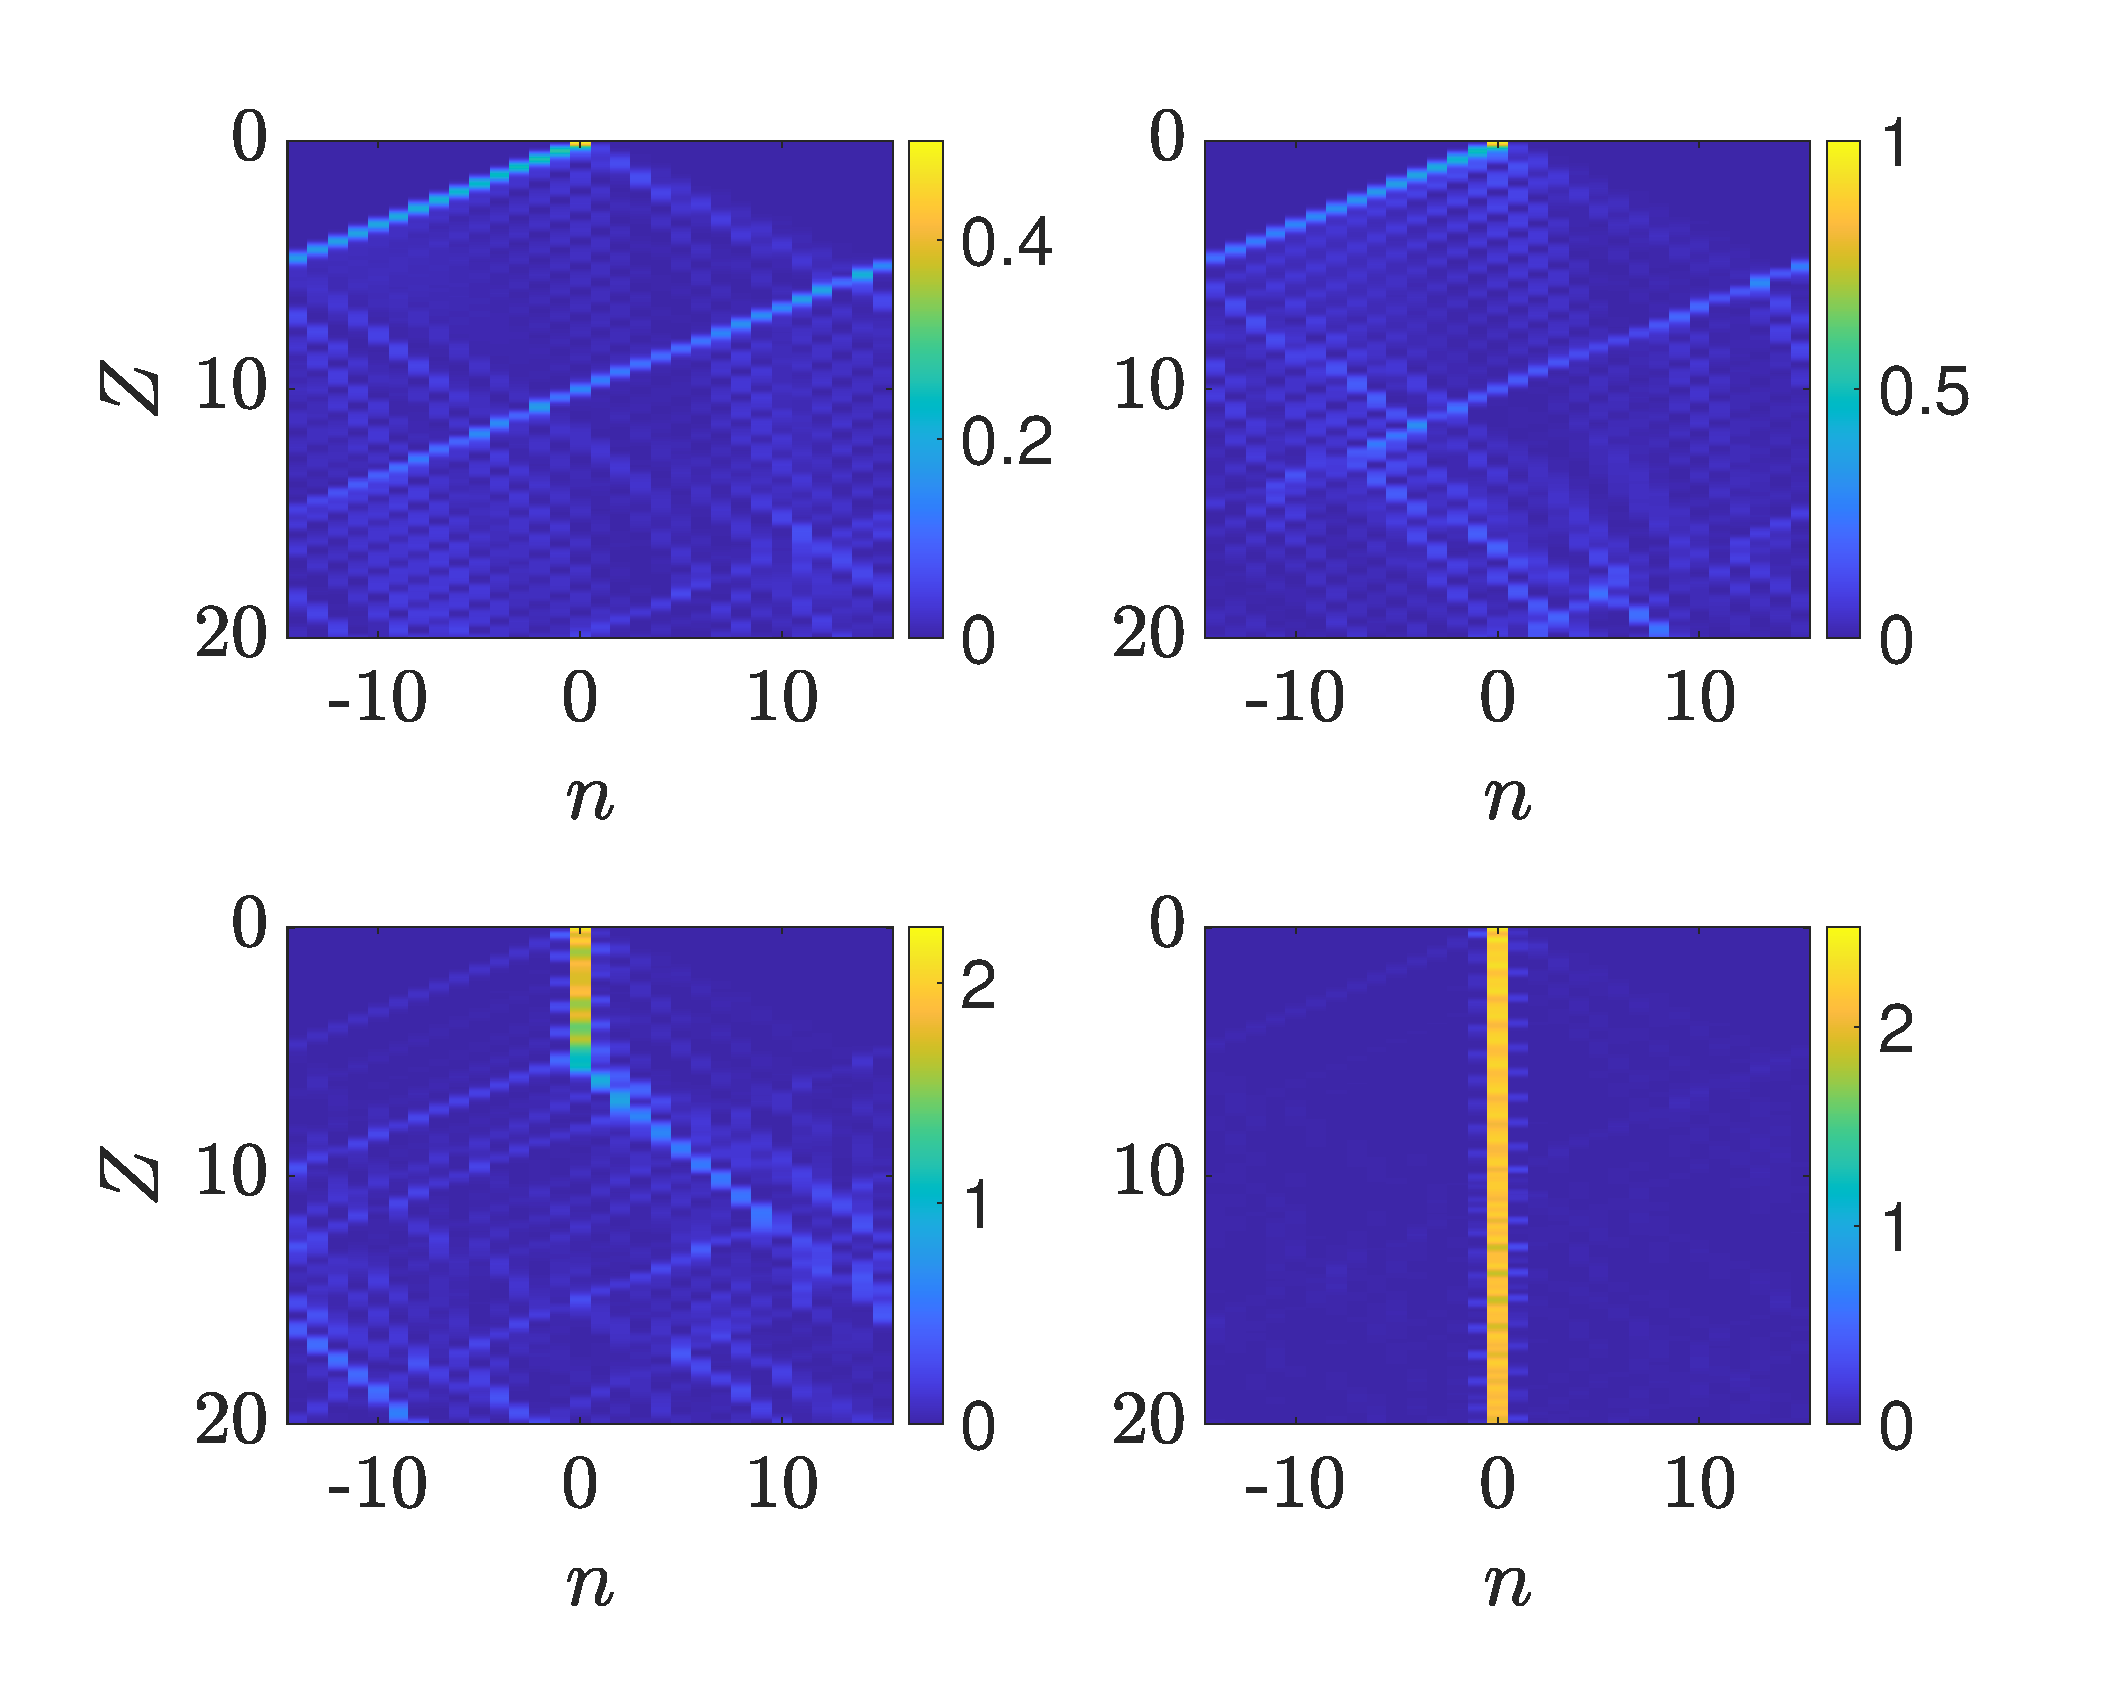
\includegraphics[width=9cm]{timestep0.eps}
    \caption{Colormap showing power of solution of equation \cref{eq:modelZ} evolving in $Z$, starting with a single excited site at $n=0$ with power $P=0.5,1,2.25,2.5$ (left to right, top to bottom). }
    \label{fig:timestep0}
\end{figure}

\begin{figure}
    \centering
    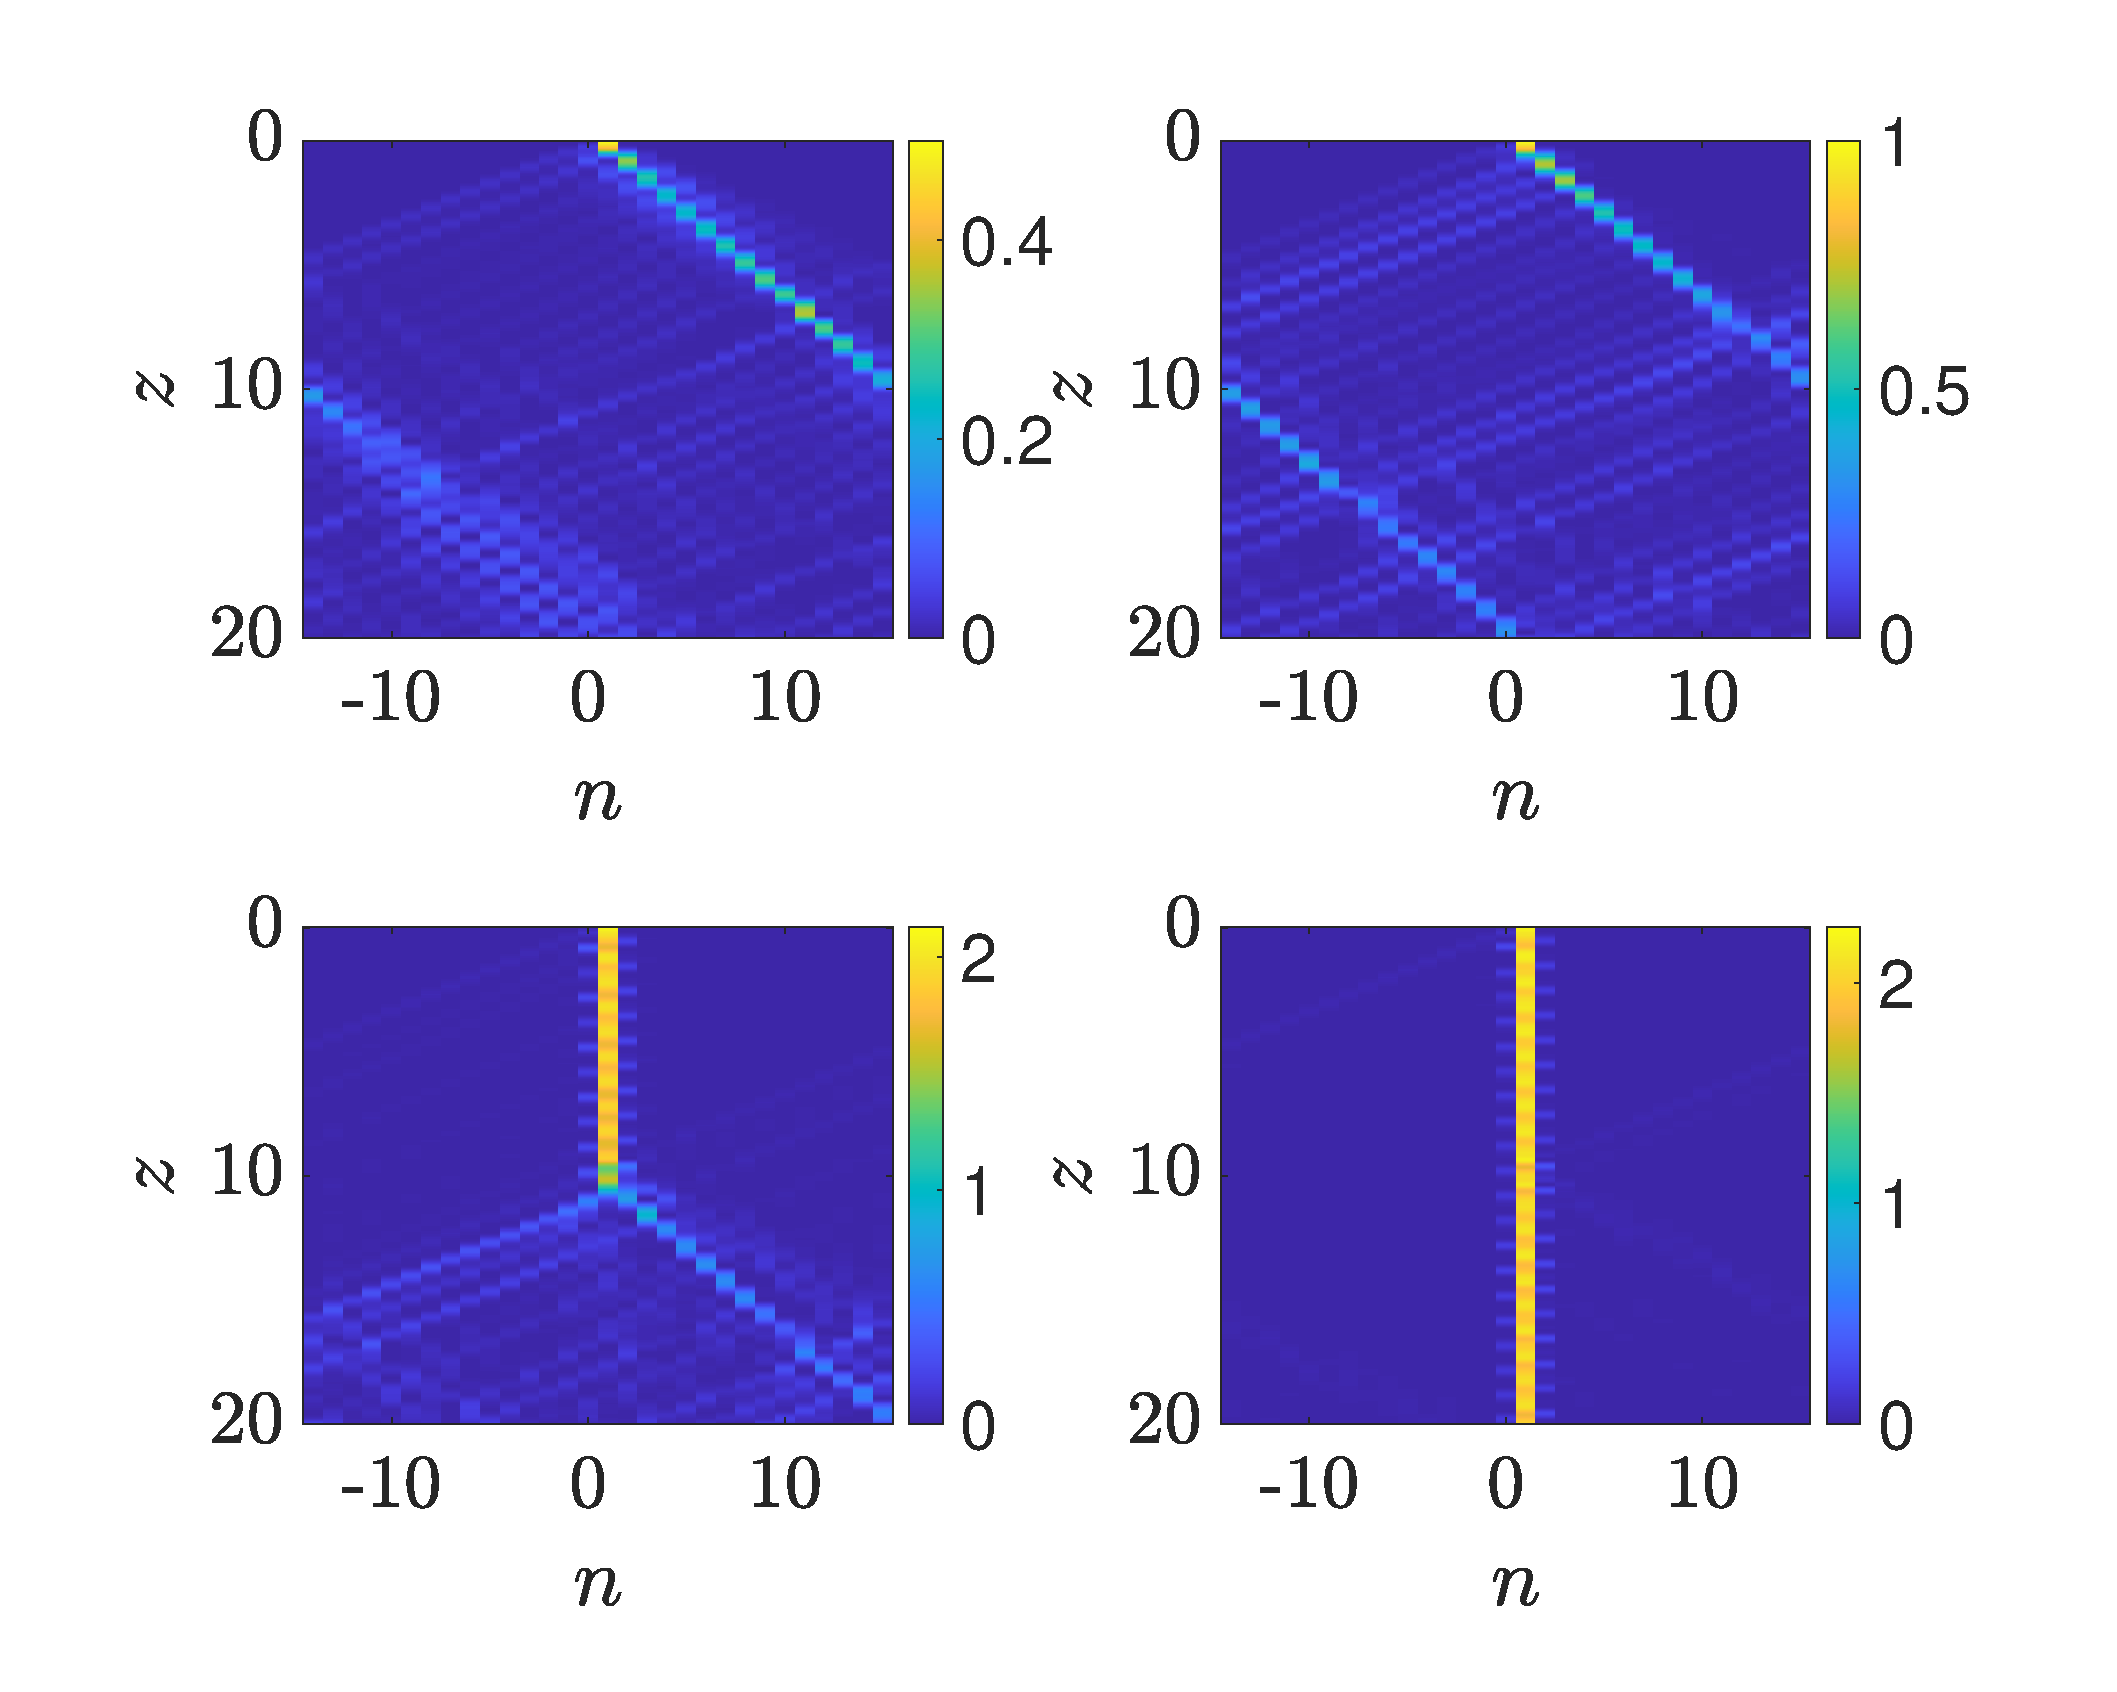
\includegraphics[width=9cm]{timestep1.eps}
    \caption{Colormap showing power of solution of equation \cref{eq:modelZ} evolving in $Z$, starting with a single excited site at $n=-1$ with power $P=0.5,1,2.15,2.25$ (left to right, top to bottom).}
    \label{fig:timestep1}
\end{figure}

A heuristic explanation of these different behaviors can be found by considering the simplification of the system \cref{eq:model} obtained by approximating the coupling functions $J_n(Z)$ with step functions. Specifically, we define
\begin{equation}\label{eq:simpleJn}
J_n(Z) = \begin{cases}
C\chi_{[0,1/3]}(Z) & Z \equiv 2 \text{ (mod 3)} \\
C\chi_{[1/3,2/3]}(Z) & Z \equiv 1 \text{ (mod 3)}\\
C\chi_{[2/3,1]}(Z) & Z \equiv 0 \text{ (mod 3)}
\end{cases}
\end{equation}
for $Z \in [0,1]$, and extend periodically for all $Z$. The function $\chi_{[a,b}](Z)$ is the characteristic function of the interval $[a,b]$, defined by
\[
\chi_{[a,b]}(Z) = \begin{cases}
1 & Z \in [a,b] \\
0 & \text{otherwise}.
\end{cases}
\]
Using this approximation, equation \cref{eq:modelZ} for $u_0$ and $u_{-1}$ on $Z \in [0,1/3]$ becomes
\begin{equation}\label{eq:approx2}
\begin{aligned}
&i \frac{1}{L} \frac{d u_0}{d Z} + C u_{-1} + |u_0|^2 u_0 = 0 \\
&i \frac{1}{L} \frac{d u_{-1}}{d Z} + C u_{0} + |u_{-1}|^2 u_{-1} = 0,
\end{aligned}
\end{equation}
where we take $g=1$ for simplicity. For $Z \in [0,1/3]$, lattice sites 0 and -1 are coupled to each other, but not to their other neighbors. 

For a low power single-site initial condition at $n=0$, the flux between the sites $n=0$ and $n=-1$ is entirely to the left, i.e. power only flows from $n=0$ to $n=-1$ (dotted line in \cref{fig:simplemodel1}, top left). A purely leftward flux is also observed when using the original coupling function (solid line in \cref{fig:simplemodel1}, top left).
For a low power single-site initial condition at $n=-1$, the flux is entirely the right (not shown).
This provides a heuristic explanation for why moving solutions result from evolution of low-power initial conditions; in both cases, there is unidirectional flow of power in a direction dictated by the active coupling.

\begin{figure}
    \centering
    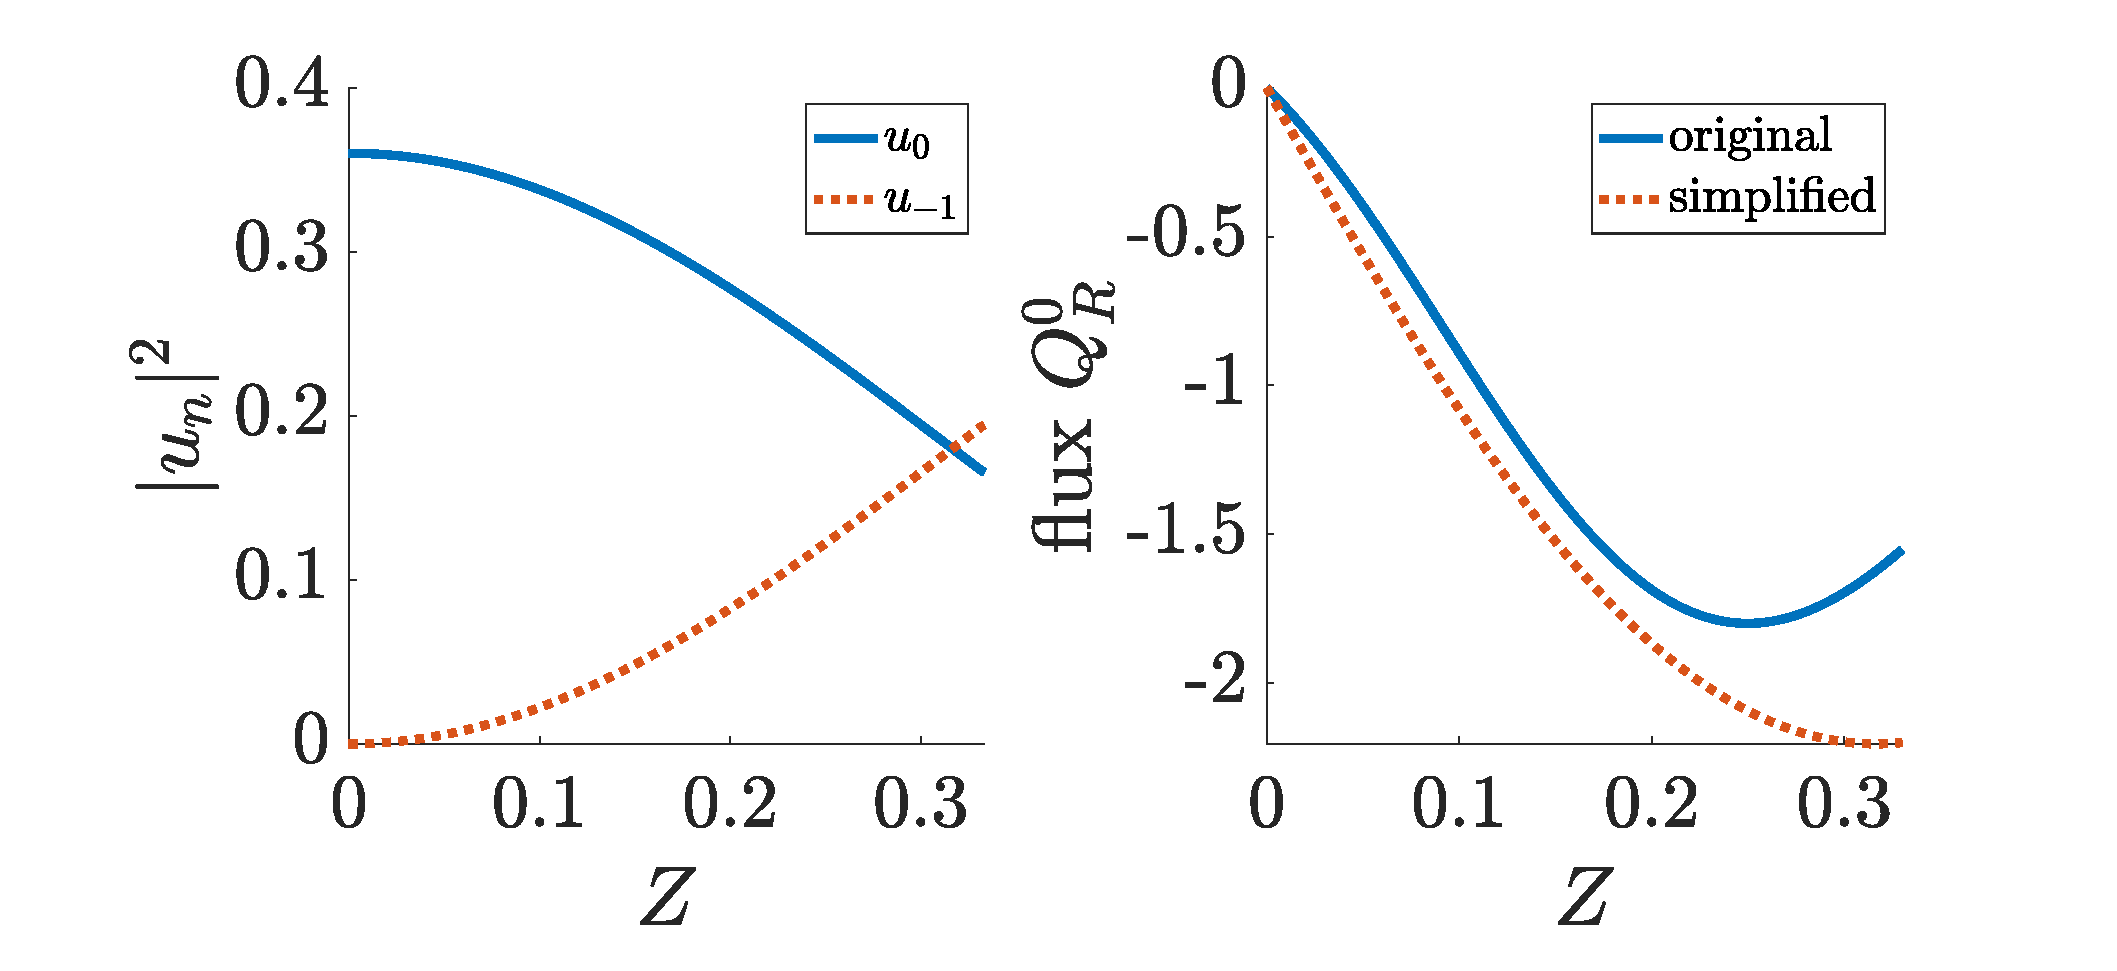
\includegraphics[width=9cm]{simplemodelL06.eps}
    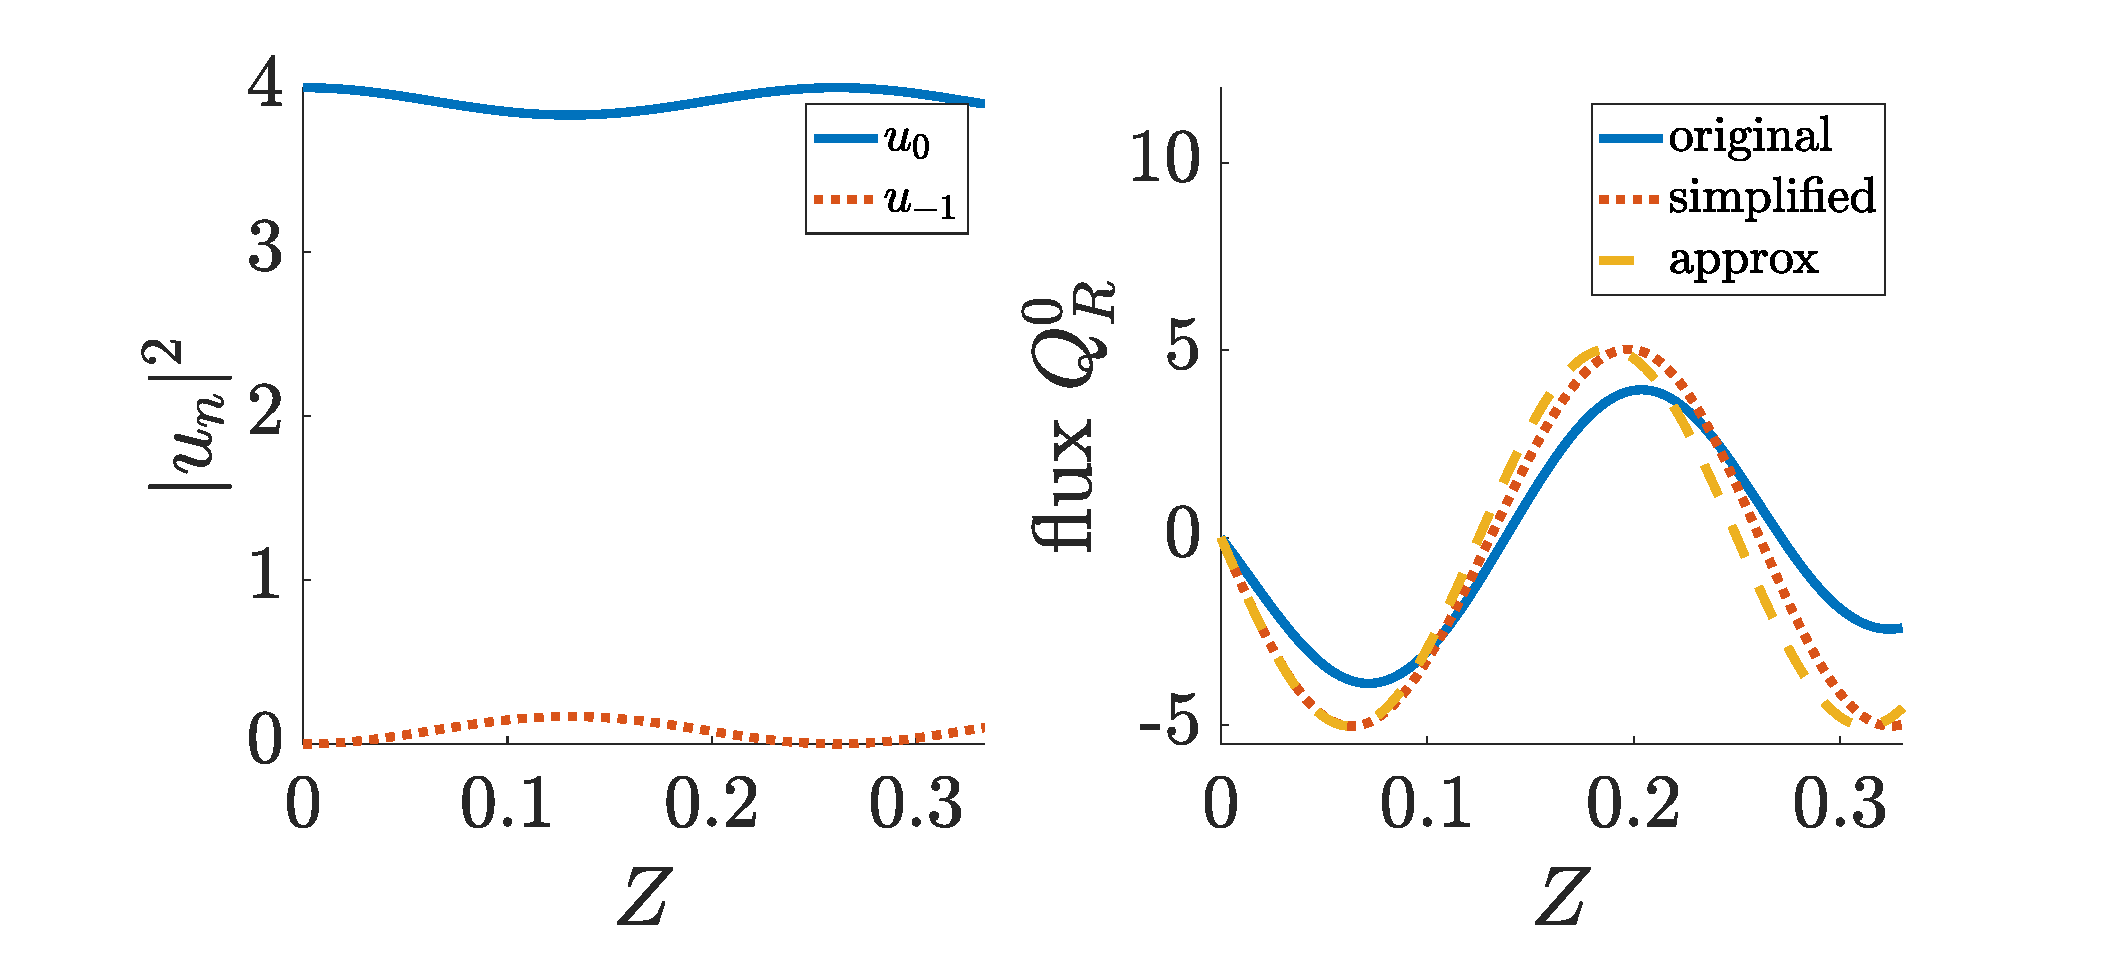
\includegraphics[width=9cm]{simplemodelstat2.eps}
    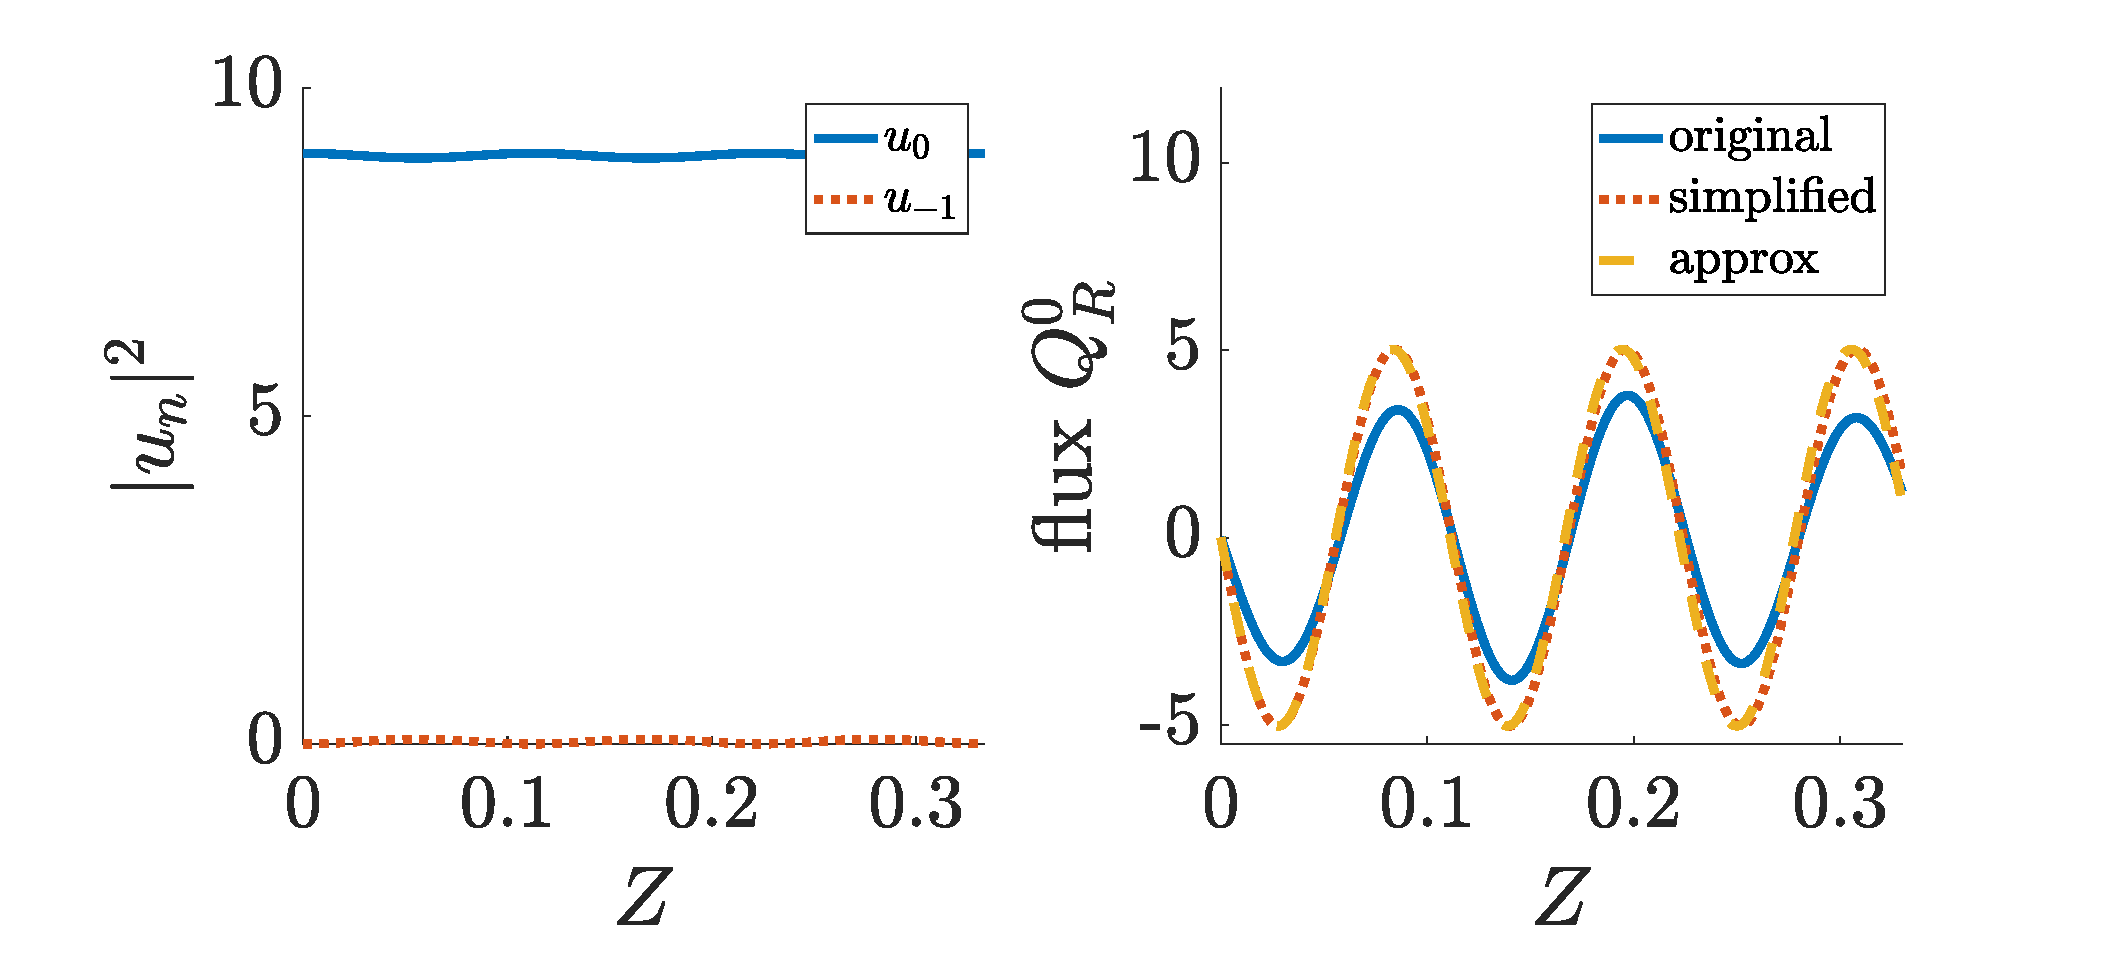
\includegraphics[width=9cm]{simplemodelstat3.eps}
    \caption{Left: power of sites 0 and -1 for evolution of model with simplified coupling function \cref{eq:simpleJn}. Right: leftward flux $Q_L^0$ at site 0 (right) for original coupling function and simplified coupling function. Evolution starts with single-site initial condition with power $|U_0(0)|^2$ of 0.36 (top), 4 (middle), and and 9 (bottom). For middle and bottom plots, approximate flux for simplified coupling function is given by \cref{eq:approxLflux}.}
    \label{fig:simplemodel1}
\end{figure}

To explain the observation that large initial power yields stationary solutions, 
we make the assumption that the central site is a pure standing wave solution $u_0(Z) = A_0 e^{2 \pi i A_0^2 Z}$ (any deviations from this are assumed to be small), and that the intensity of the neighboring site $u_{-1}$ is small. (Numerical experiments demonstrate that this is indeed the case, to leading order; see \cref{fig:stat3}). Since we are assuming $u_{-1}$ is small, we neglecting the nonlinear term in the second equation in \cref{eq:approx2} to obtain the approximation
\begin{equation}
\frac{d u_{-1}}{d Z} = i C L A_0 e^{2 \pi i A_0^2 Z},
\end{equation}
which we can solve to obtain
\begin{align}
u_{-1}(Z) &= \frac{CL}{2\pi A_0}\left( e^{2\pi i A_0^2 Z} - 1\right) 
&& Z \in [0,1/3],
\end{align}
where we took the initial condition $u_{-1}(0) = 0$.
The leftward flux $Q_0^L(Z)$ at the central site $n=0$ is then given by
\begin{align}\label{eq:approxLflux}
Q_0^L(Z) &= -\frac{C L^2}{\pi} \sin\left(2 \pi A_0^2 Z \right),
\end{align}
which is oscillatory with frequency $A_0^2$. See \cref{fig:simplemodel1} (middle and bottom) for a comparison between the flux computed by solving the system of ODEs \cref{eq:modelZ} using the simplified coupling function \cref{eq:simpleJn} and the approximation \cref{eq:approxLflux}. (The rightward flux at the neighboring site $n=-1$ is equal and opposite to this). For the original coupling function, the flux is also oscillatory with similar frequency (solid lines in left panel of \cref{fig:simplemodel1}, middle and bottom). The approximate net leftward flux $Q_{L}^0([0,1/3])$ for the central site over the interval $Z \in [0, 1/3]$ is found by integrating \cref{eq:approxLflux} to get
\begin{equation}\label{eq:approxflux}
Q_{L}^0([0,1/3]) = -\frac{CL^2}{A_0^2\pi^2}\sin^2\left( \frac{\pi A_0^2}{3}\right).
\end{equation}
We note that while the approximate net leftward flux \cref{eq:approxflux} in fact 0 for particular values of $A_0$, what is much more important is that is this small for large $A_0$, which is a consequence of averaging an oscillatory function over a finite interval. Thus, although power flows back and forth from sites 0 and -1 over the interval $Z \in [0, 1/3]$, the net flux is very small for large initial power (both for the original and the simplified coupling functions), which explains the observation of stationary solutions for high power, single-site initial conditions.

\section{Coherent structures}

These evolution experiments suggest that the system \cref{eq:modelZ} supports two classes of coherent structures: stationary solutions, which are centered at a single lattice site, and moving solutions, which reproduce themselves exactly a specific number of sites to the left or to the right. Recall that for the rescaled system \cref{eq:modelZ}, the coupling period is 1. The stationary coherent structures will be periodic orbits whose period is a multiple of the coupling period, i.e. a positive integer. We note that while it may be possible to find such solutions which have a noninteger period, Floquet analysis requires that the period of the solutions be commensurate with that of the coupling. Similarly, we will look for moving solutions that reproduce themselves, shifted left or right, after an integer period.

For appropriate choices of system parameters, we can compute both types of solutions numerically. For both stationary and moving solutions, we use a shooting method with periodic boundary conditions imposed on $Z$, starting with a single-site initial guess. In addition, for stationary solutions, we validate this method by using numerical parameter continuation with AUTO \cite{auto07p} to solve a periodic boundary value problem. Unless otherwise specified, the parameters in the section are the same as in the previous section. 

\subsection{Stationary solutions}

First, we look at the stationary solutions. At the anti-continuum (AC) limit ($J=0$ and $C=0$), the lattice sites are decoupled, and an initial power $P$ at lattice site $n$ will yield a standing wave solution of frequency $P$, i.e. of the form $u_n(Z) = \sqrt{P} e^{ 2 \pi i P Z}$. Since such a solution has period $1/P$, and stationary solutions must have an integer period, these solutions will exist in a discrete family for every integer period $N$, i.e. approximately $P = k/N$ for sufficiently large positive integer $k$. For period $N=1$ and the parameters in the previous section, for example, we expect have stationary solutions for approximate integer powers $P \geq 2$. See \cref{fig:stat2} and \cref{fig:stat3} for the first two of these solutions. By looking at the power and the real part of the central site ($n=0$), we see that it is approximately a standing wave with frequency 2 and 3 (respectively). We note that the stationary solutions do not decay to 0 with increasing $|n|$, but rather the tails exhibit small amplitude oscillatory patterns (see top right of \cref{fig:stat2} and \cref{fig:stat3}); the specific pattern of oscillations depends on the lattice size (not shown).
Looking at the sites adjacent to the central site, the left neighbor $u_{-1}$ peaks on the interval $[0,1/3]$ when the coupling $J_2(z)$ is most active, and the leftward flux at the central site is negative (indicating flow of power to the left). The right neighbor peaks on the interval $[2/3, 1]$ when the coupling $J_0(z)$ is most active and the rightward flux at the central site is negative (indicating flow of power to the right). Both leftward and rightward fluxes are close to 0 on the interval $[1/3, 2/3]$, when neither nearest-neighbor coupling is strong.

\begin{figure}
    \centering
    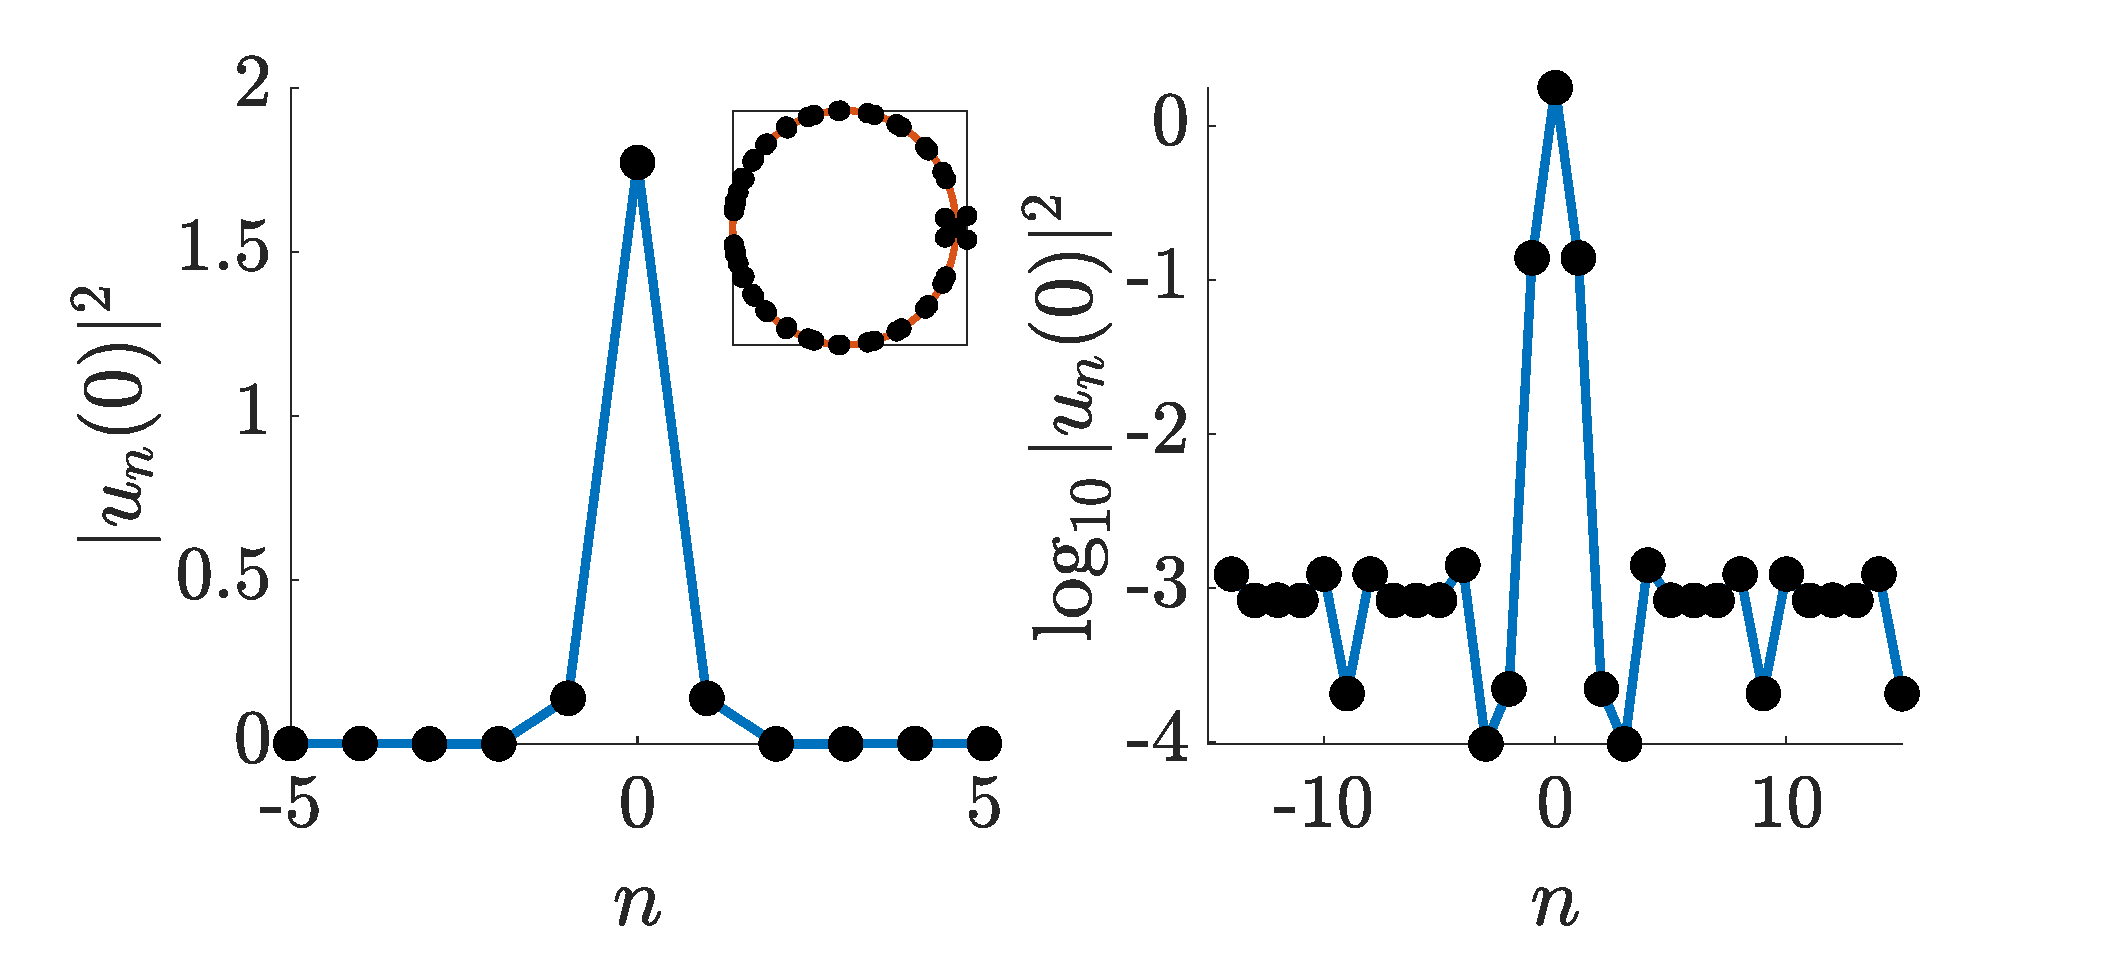
\includegraphics[width=9cm]{stat2a.eps}
    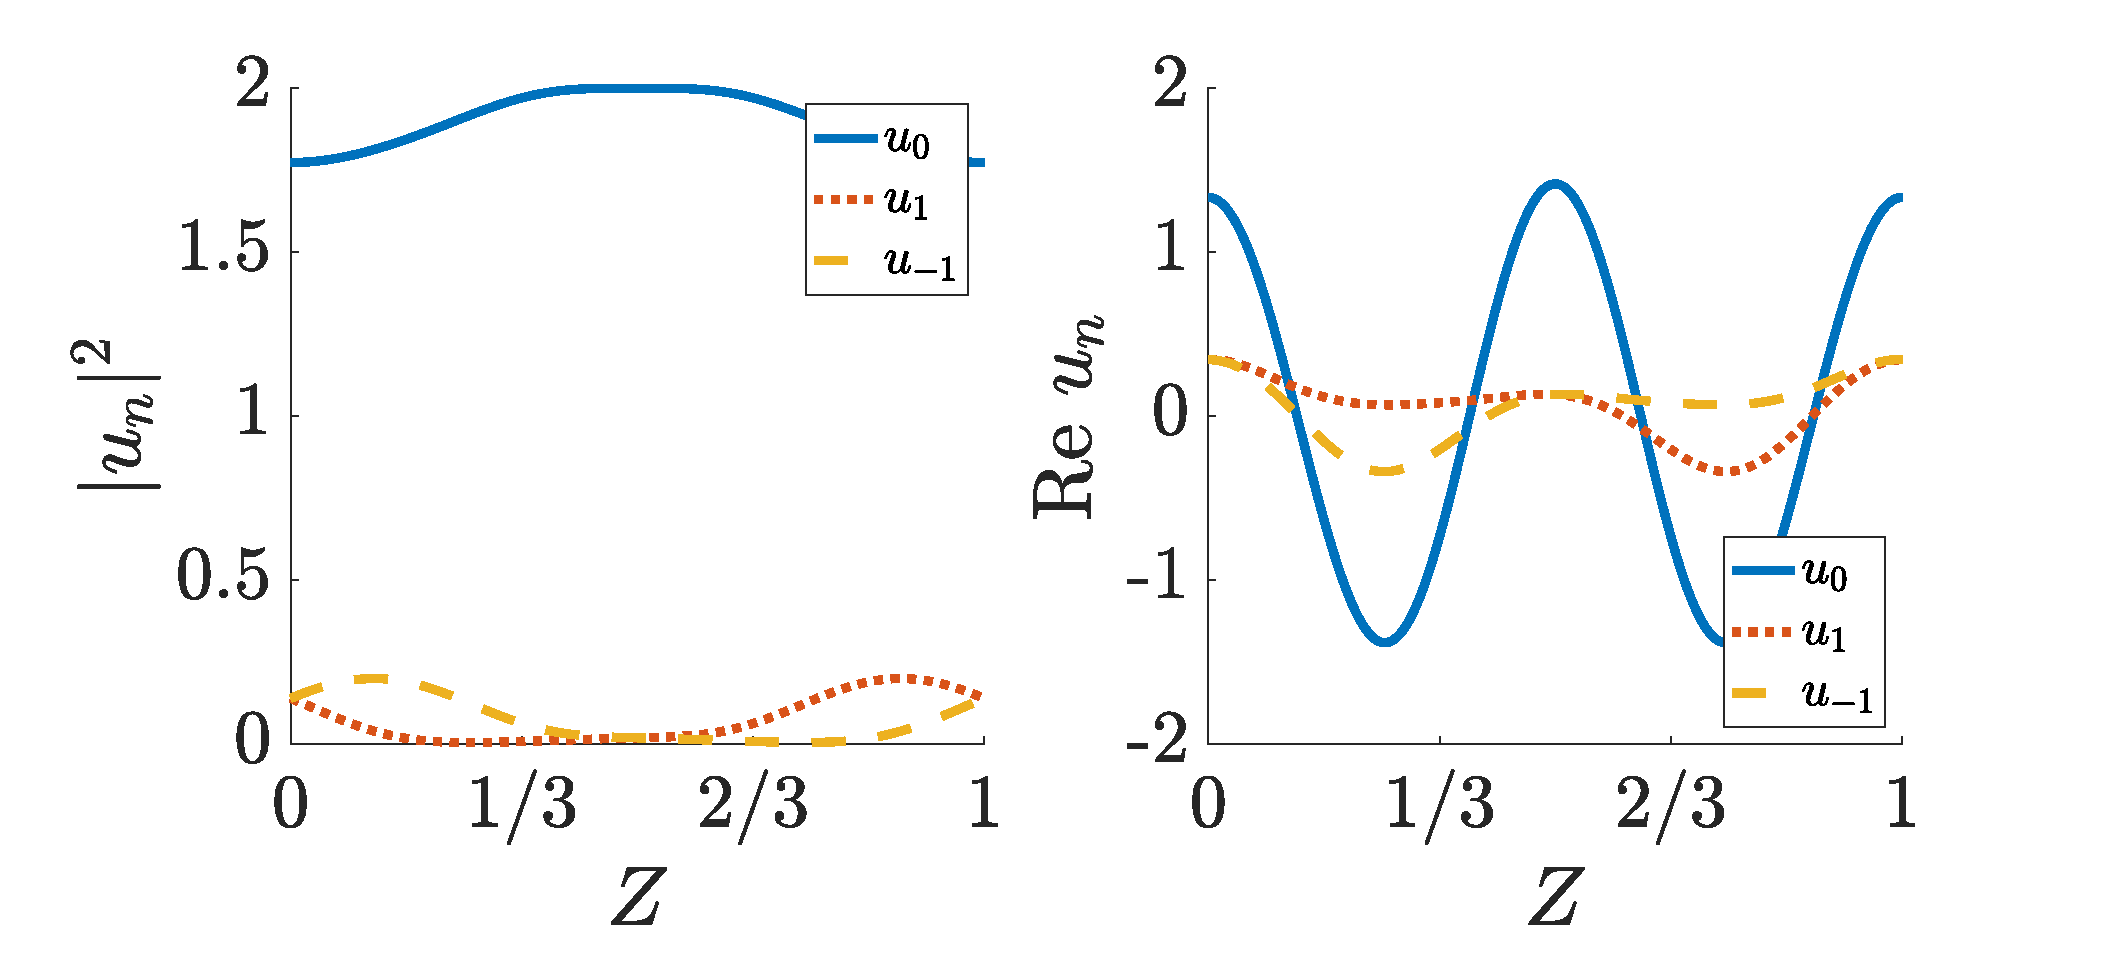
\includegraphics[width=9cm]{stat2b.eps}
    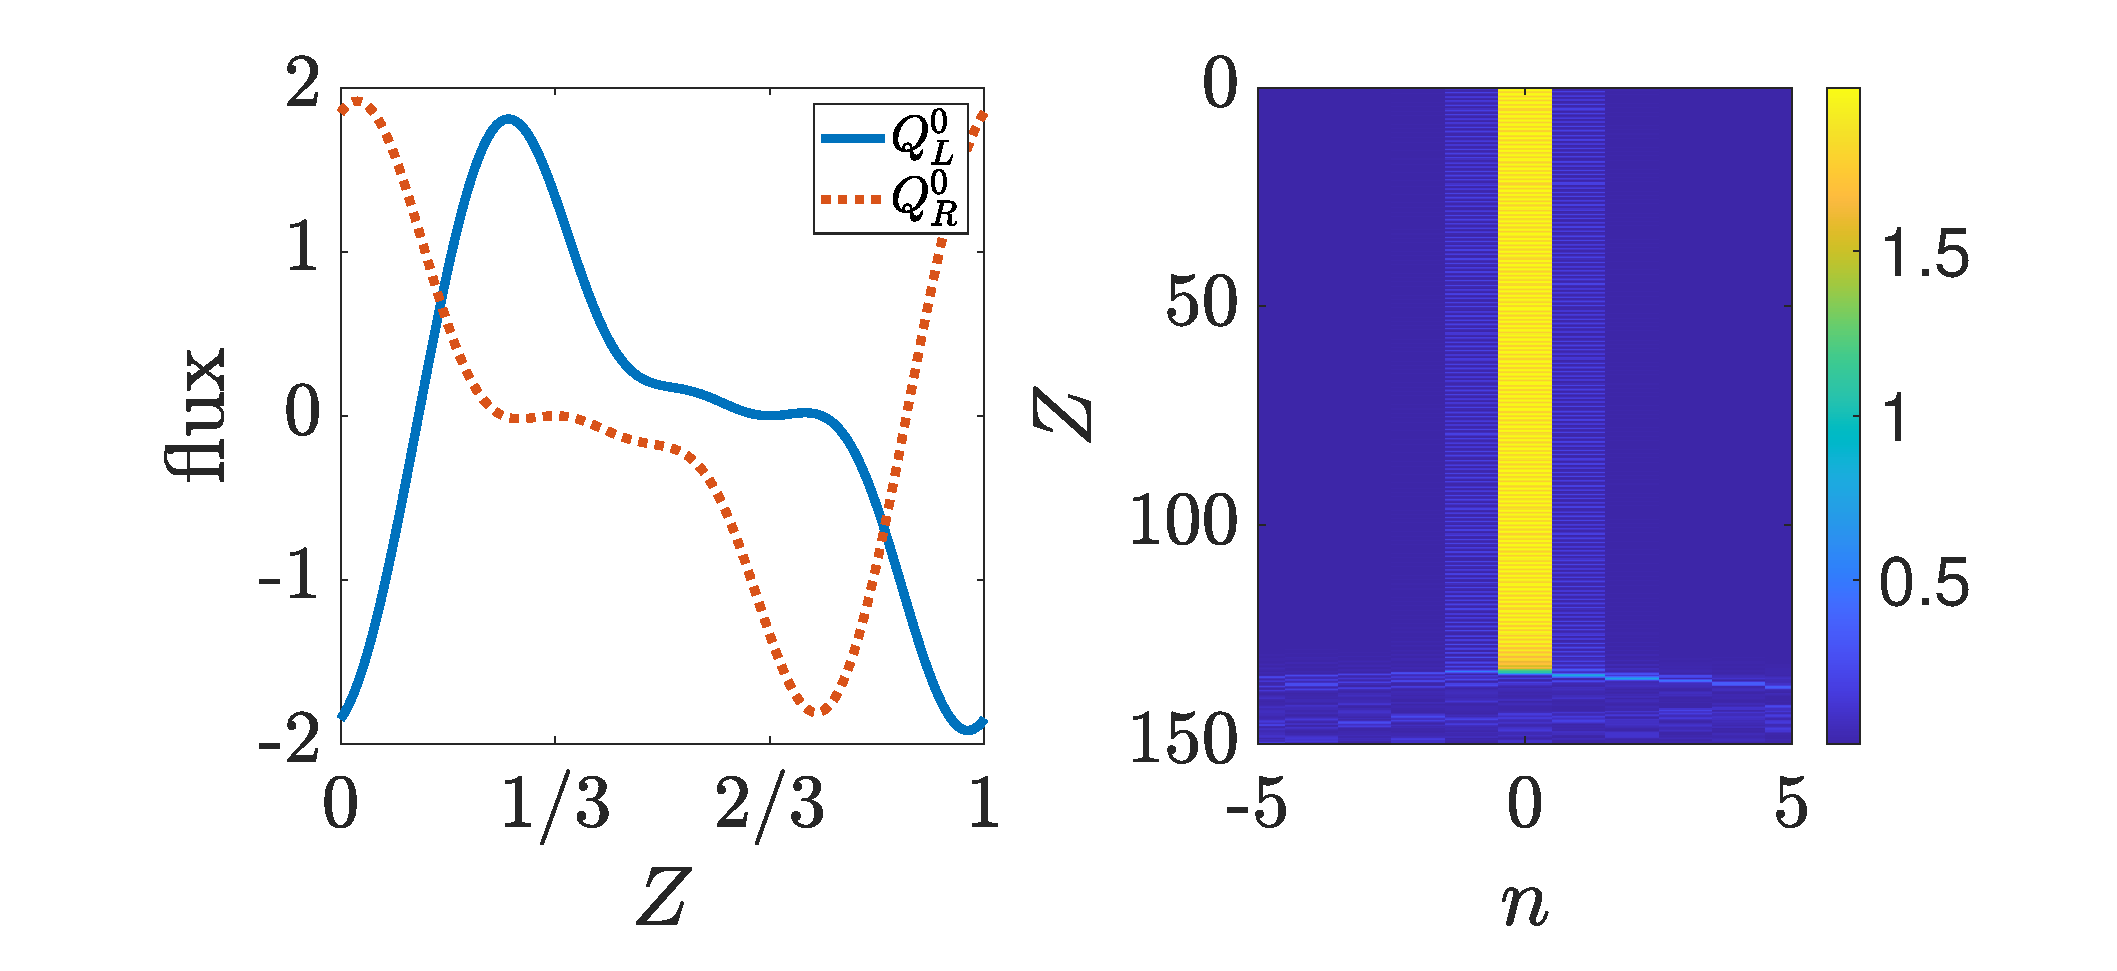
\includegraphics[width=9cm]{stat2c.eps}
    \caption{Top: initial power $|u_n(0)|^2$ (left) with inset showing Floquet multipliers, and log of initial power (right) for stationary solution with approximate power of 2.. Middle: power (left) and real part (right) of three central sites over one period. Bottom: Left and right fluxes at central site $n=0$ (left), long term evolution in $Z$ (right). Evolution with \texttt{ode45} in Matlab with step size $10^{-2}$.}
    \label{fig:stat2}
\end{figure}

\begin{figure}
    \centering
    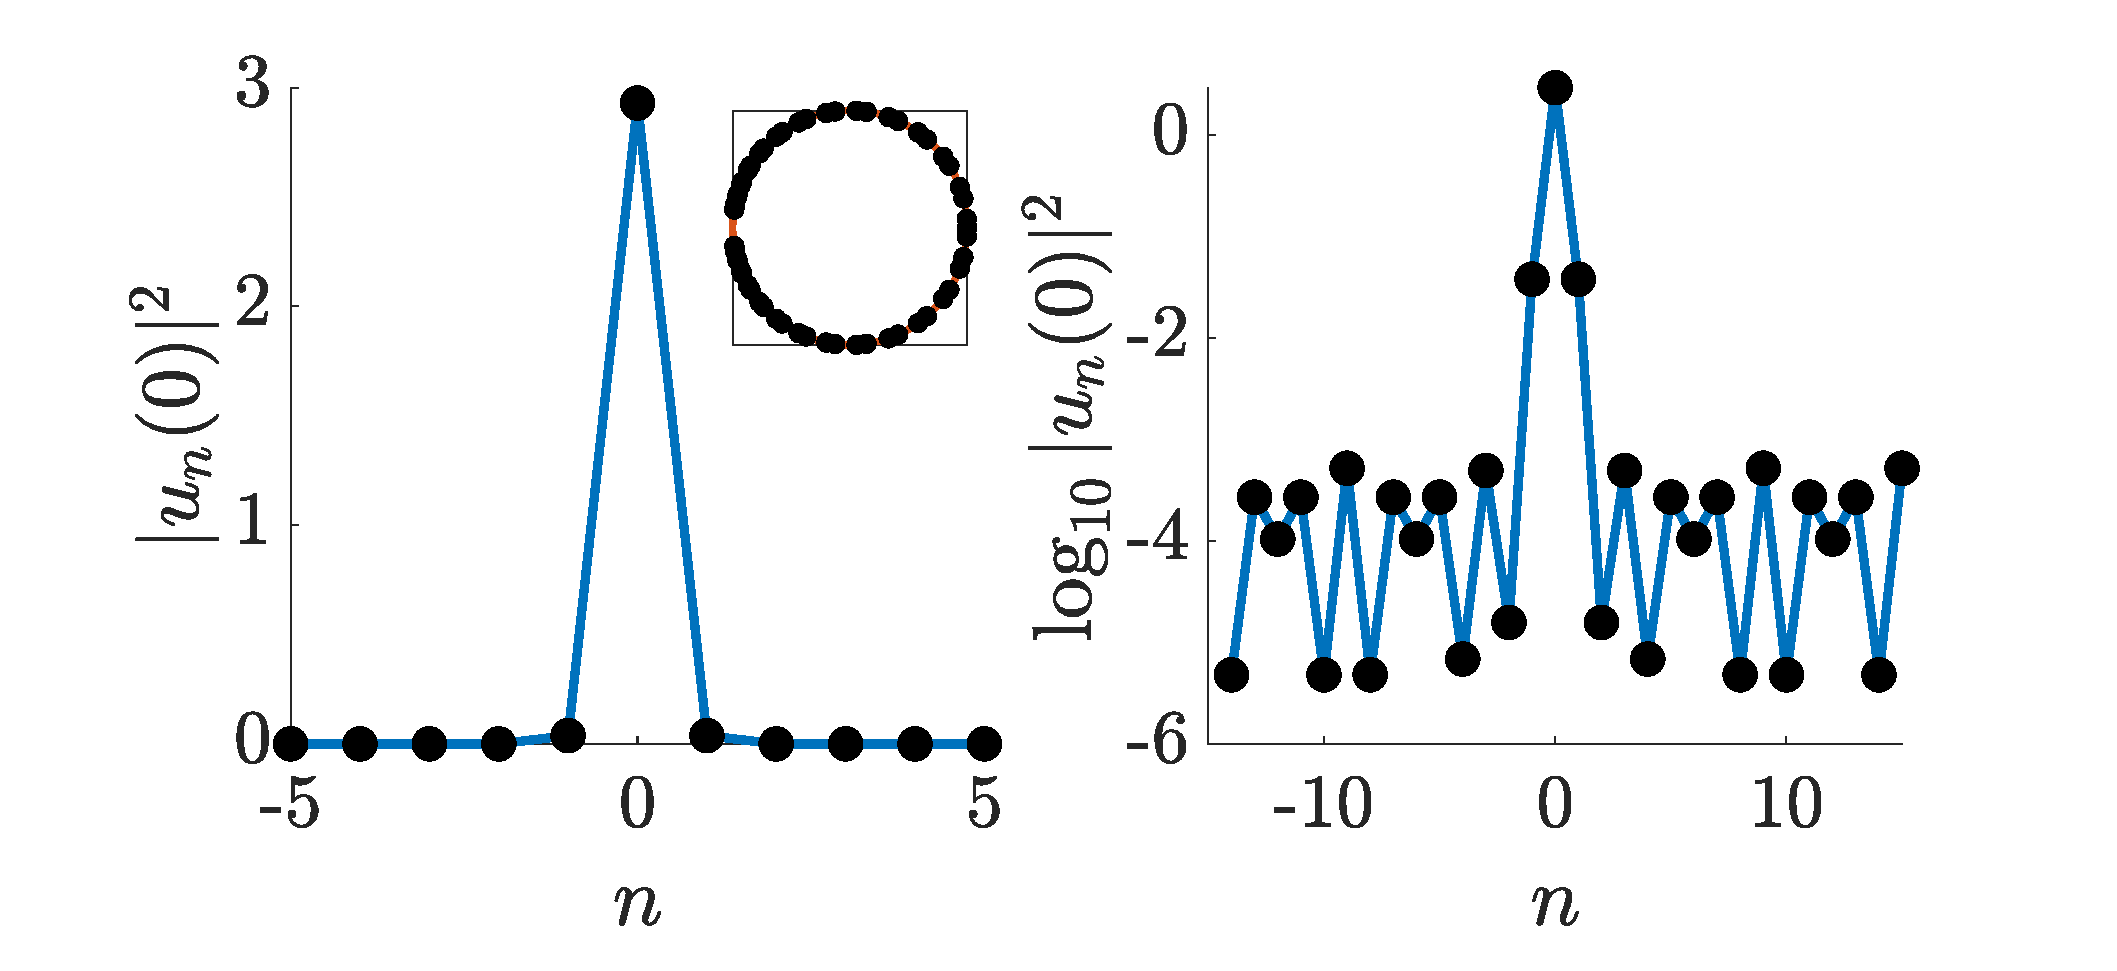
\includegraphics[width=9cm]{stat3a.eps}
    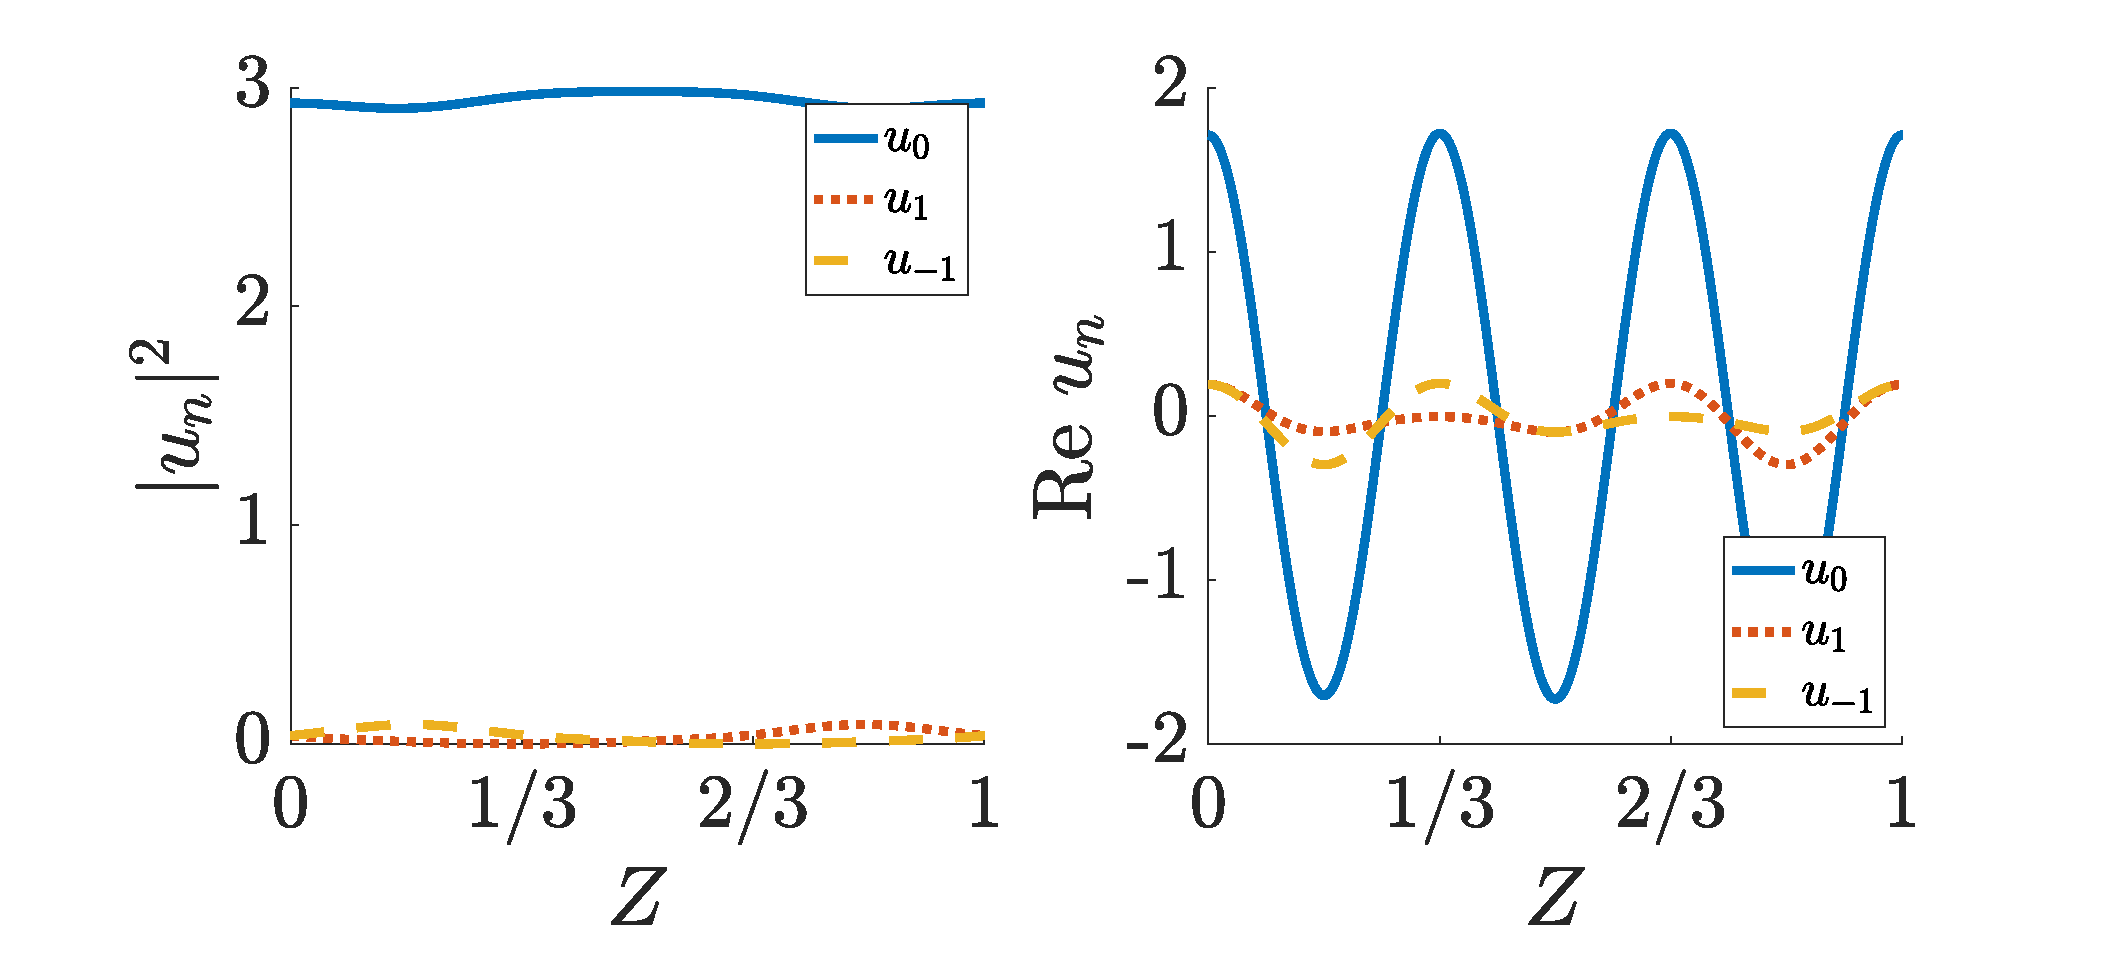
\includegraphics[width=9cm]{stat3b.eps}
    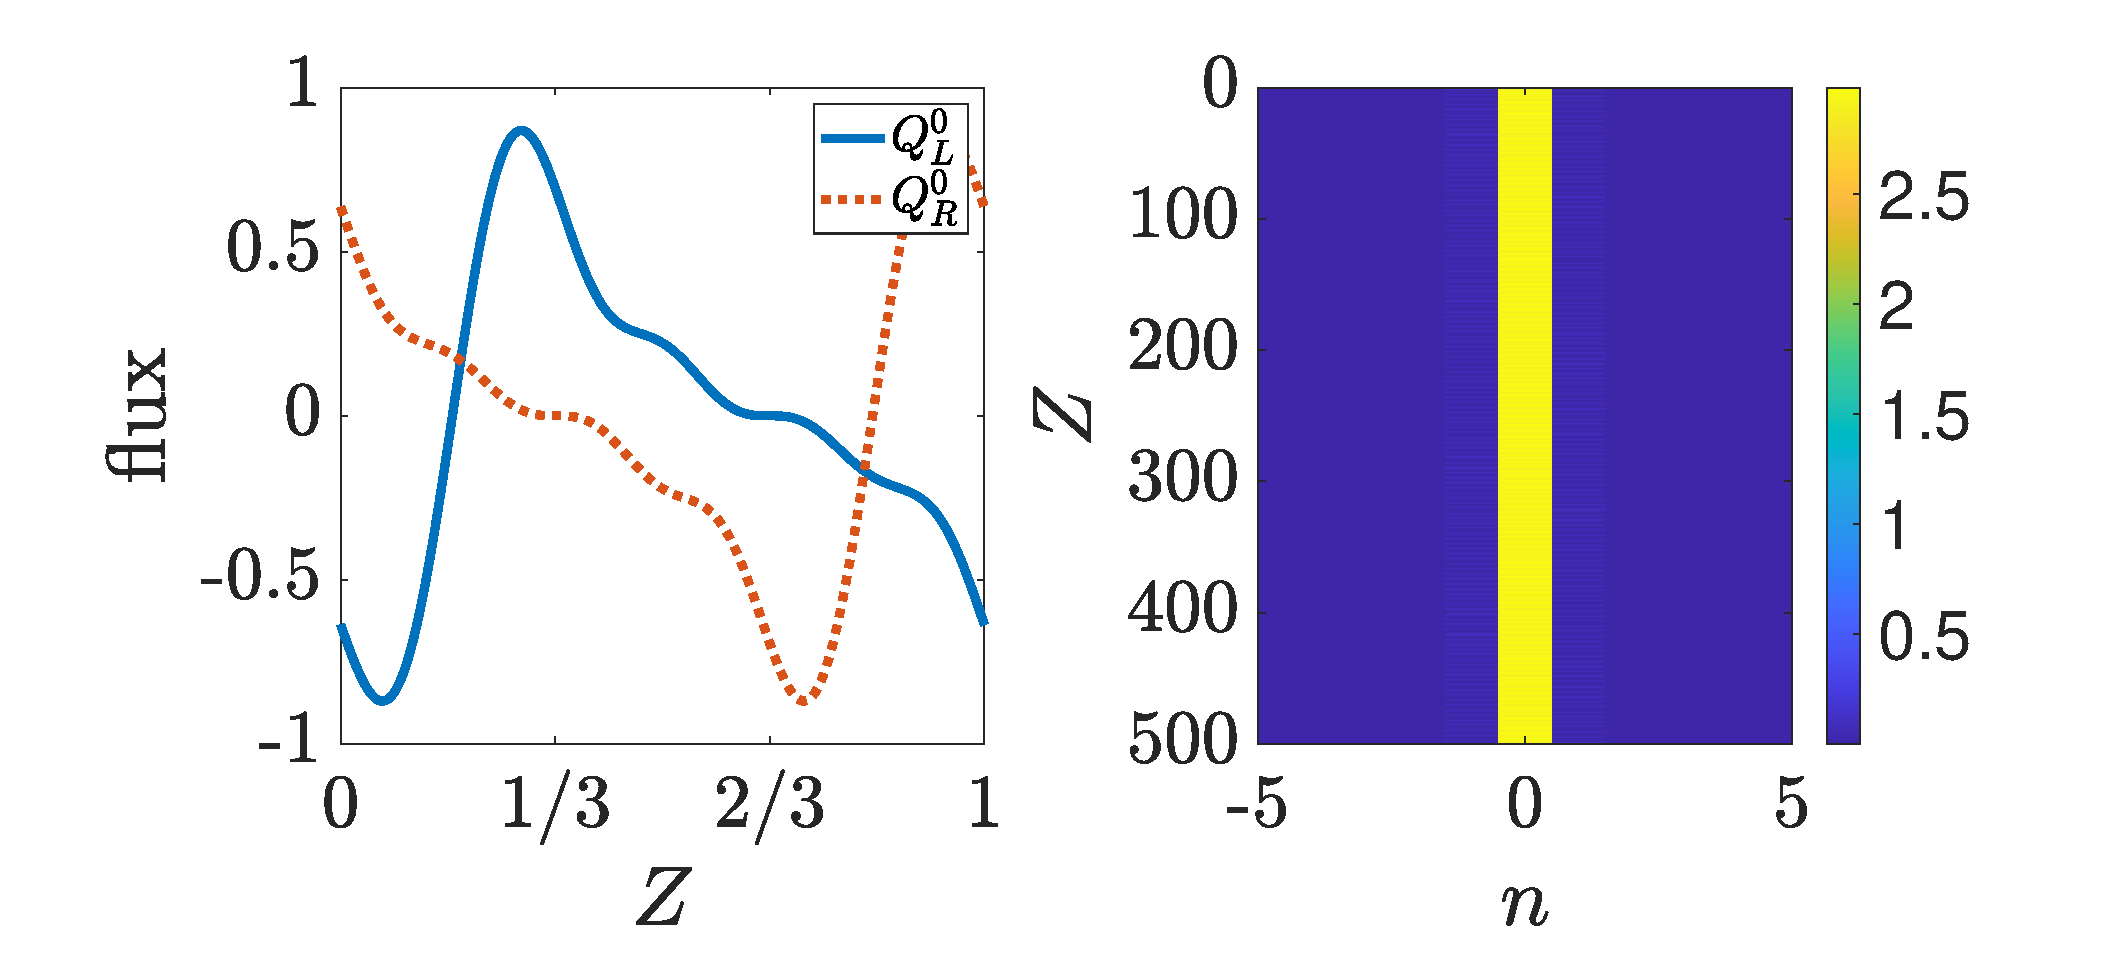
\includegraphics[width=9cm]{stat3c.eps}
    \caption{Same as \cref{fig:stat2}, but for stationary solution with approximate power of 3.}
    \label{fig:stat3}
\end{figure}

Since these stationary solutions are true periodic orbits with integer period, so that their period is equal to or commensurate with that of the coupling, their spectral stability can be determined by Floquet theory. Numerical computation of the Floquet multipliers of the stationary solutions is shown in insets of the top left plots in \cref{fig:stat2} and \cref{fig:stat3}. The lower power solution has two pairs of Floquet multipliers off of the unit circle, which is characteristic of an oscillatory instability. Long term evolution in $Z$ (bottom right plots of \cref{fig:stat2} and \cref{fig:stat3}) shows that this solution remains coherent until approximately $Z=130$. By contrast, the Floquet spectrum of the higher power solution lies on the unit circle, indicating spectral stability. Long term evolution in $Z$ shows that this solution is still coherent at $Z=500$.

Using parameter continuation, we start with the DNLS soliton at $C=0$ and slowly vary $C$, tracing the curves in \cref{fig:statAC} ($J_0 = 0.05$ throughout). Since we are looking for solutions with period 1, the starting power must take integer values so that the frequency of the DNLS standing wave at $C=0$ is commensurate with this period. In all cases, a turning point is reached, at which point the parameter continuation reverses direction. This turning point is at a larger value of $C$ for solutions which start at a higher power at $C=0$. All stationary solutions initially have their Floquet spectrum confined to the unit circle, thus are spectrally stable. Spectral stability is lost at some point before the bifurcation point, when Floquet multipliers collide and leave the unit circle. Solutions on the upper branches of the bifurcation diagram are periodic solutions to DNLS which are not pure standing waves. To leading order, these upper solutions are the sum of two Fourier modes, as opposed to to standing waves, which are a single Fourier mode. Substituting the finite Fourier ansatz 
\[
u_n(Z) = \sum_{k=-N}^N a_{n,k} e^{2 \pi i k z}
\]
into \cref{eq:modelZ} and projecting onto each of the Fourier basis functions, we can obtain expressions for the coefficients $a_{n,k}$ for each wavenumber $k$. An FFT of the numerical solution on the upper branches suggests that the solutions at each site are composed predominantly of the modes with wavenumbers 0 and 1. Thus, to leading order, these solutions are of the form $u_n(Z) = a_{n,0} + a_{n,1} e^{2 \pi i \omega Z}$, where the coefficients $a_n^0$ and $b_n^0$ satisfy 
\begin{align*}
&J_0(a_{n+1,0}+a_{n-1,0}) + a_{n,0}^3 + 2 a_{n,1}^2 a_{n,0} = 0 \\
&J_0(a_{n+1,1}+a_{n-1,1}) + a_{n,1}^3 - w a_{n,1} + 2 a_{n,1} a_{n,0}^2 = 0.
\end{align*}
We note that if $a_{n,0} = 0$ for all $n$, the second equation reduces to DNLS, in which case the solution is a standing wave.

\begin{figure}
    \centering
    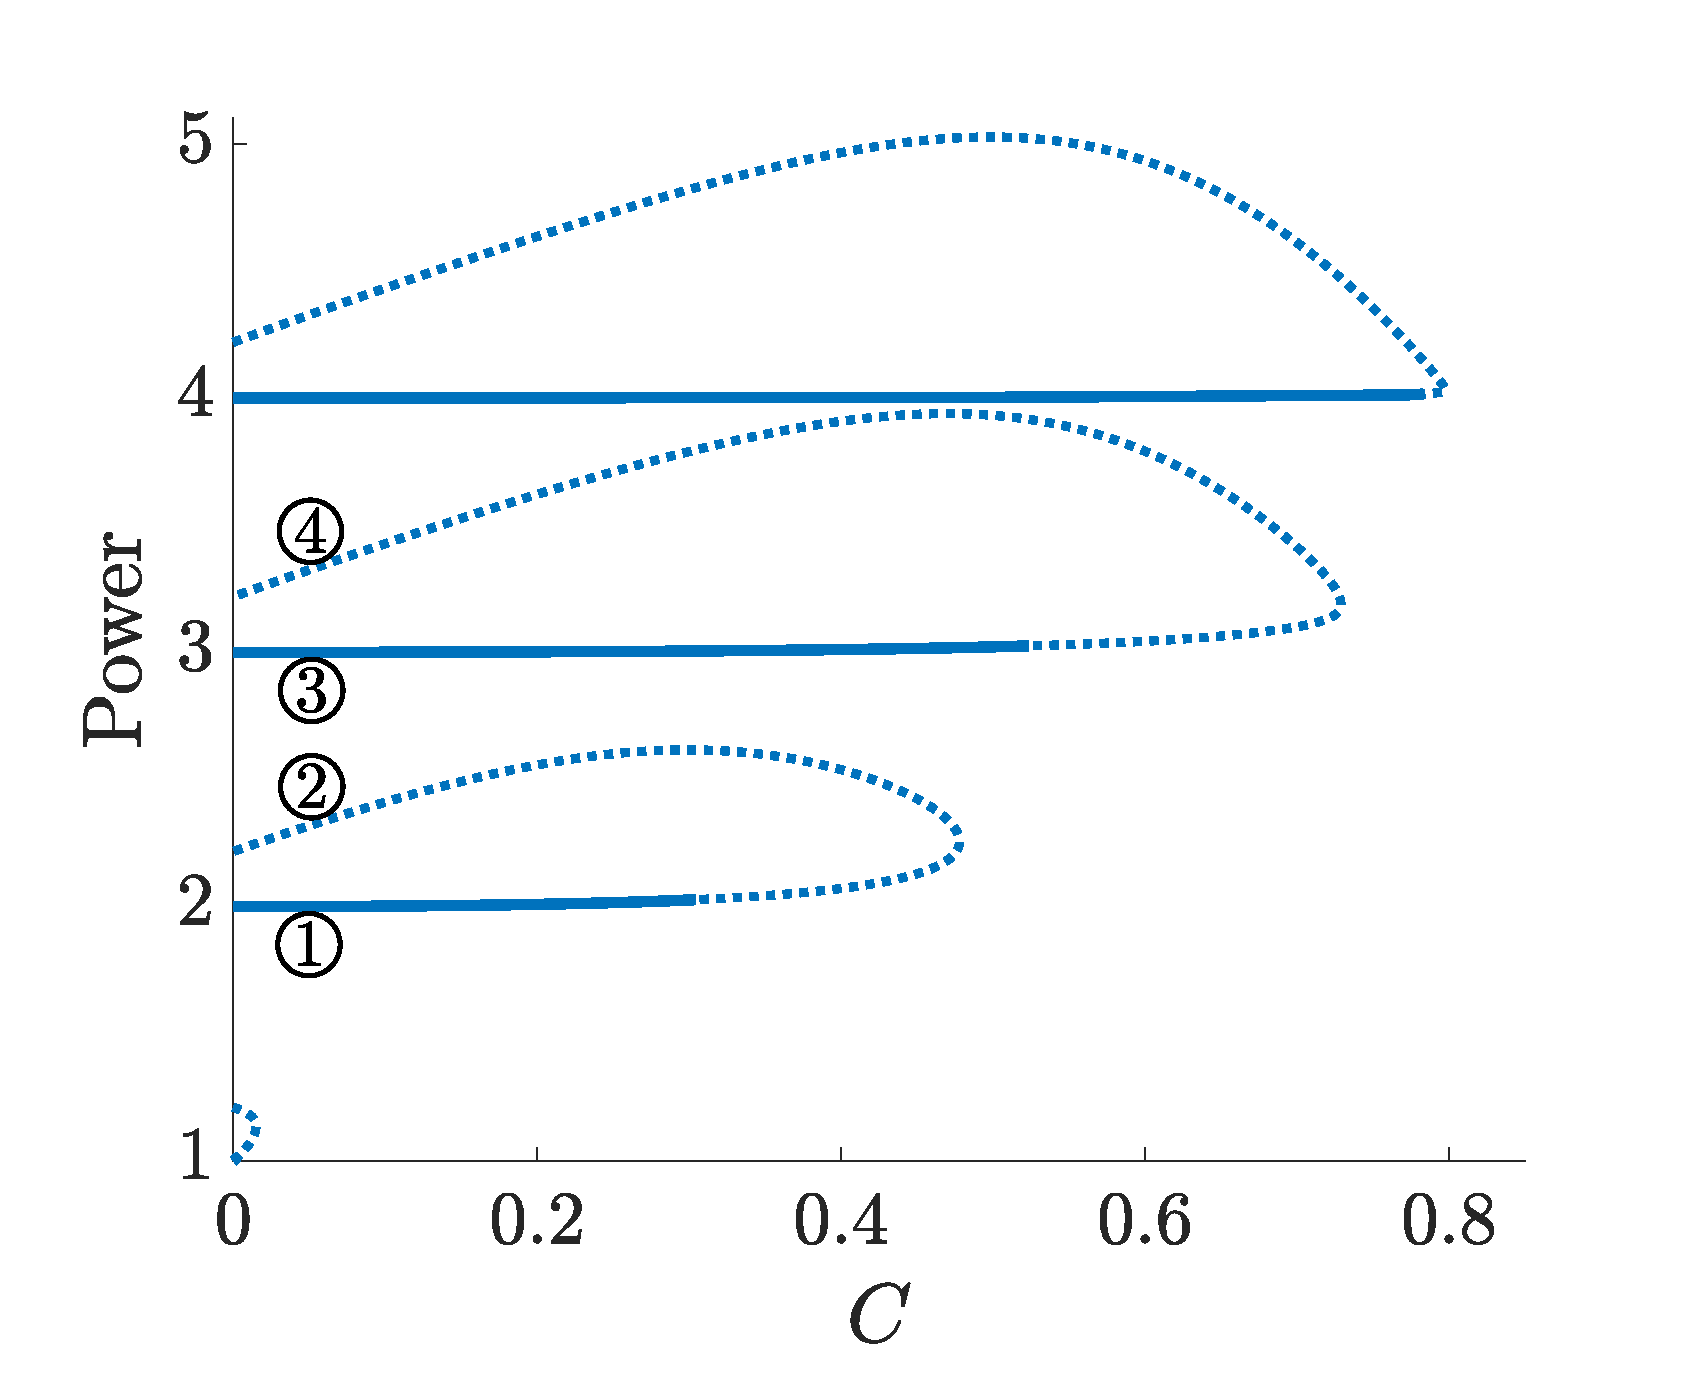
\includegraphics[width=8cm]{stat1234AC.eps}
    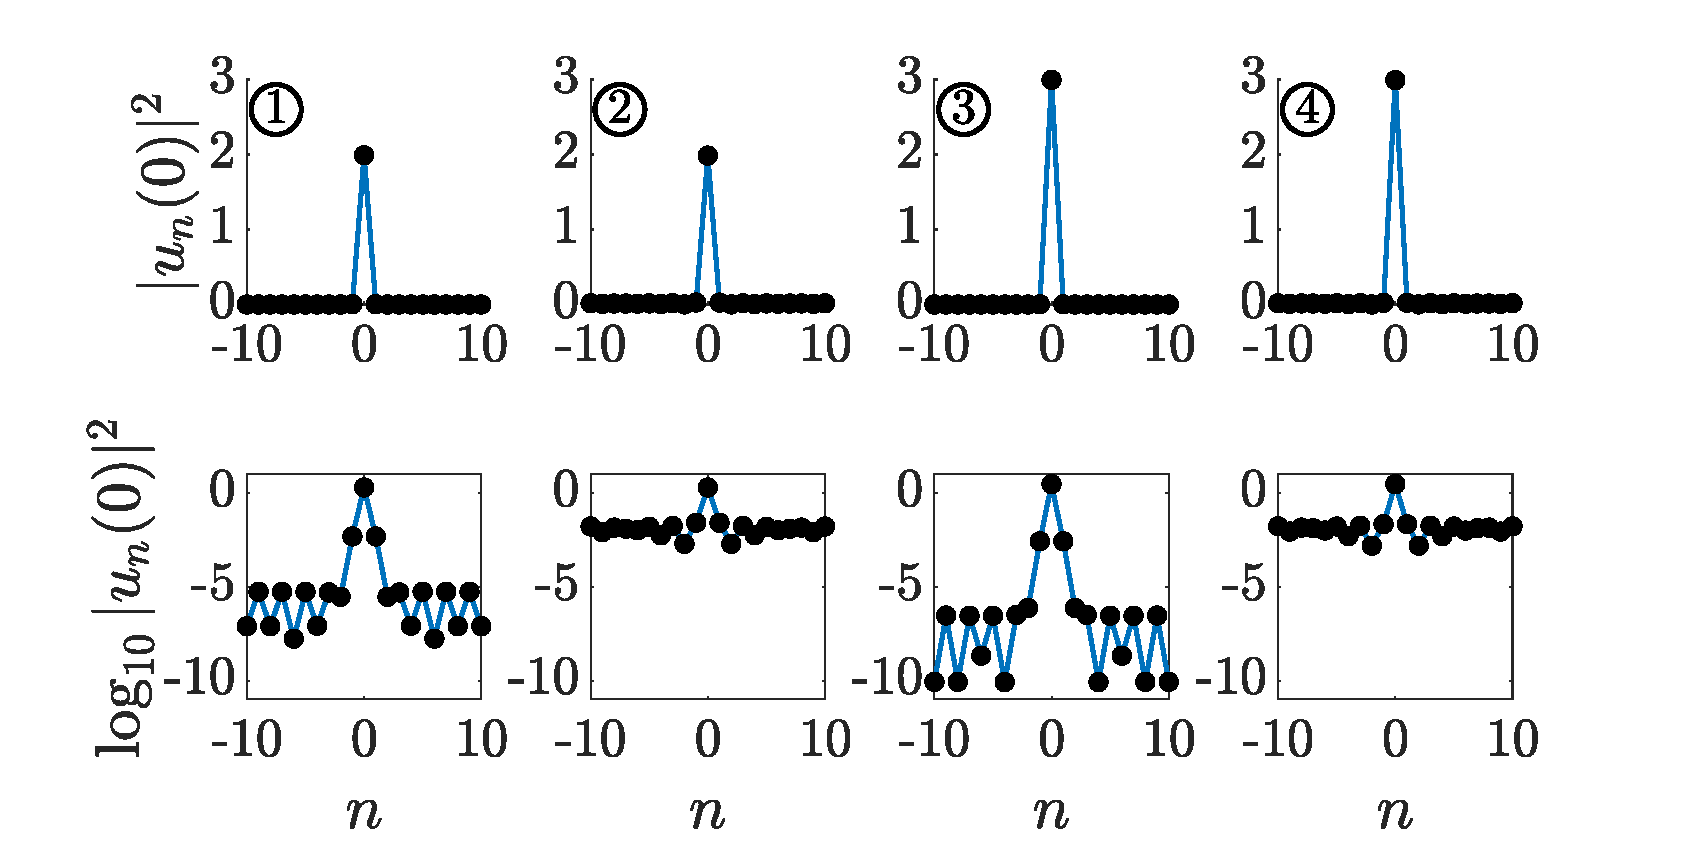
\includegraphics[width=8cm]{stat1234ACsols.eps}
    \caption{Branches of stationary solutions with period (in $Z$) of 1, obtained from numerical parameter continuation starting with DNLS soliton at $C=0$. Bottom plots show power (top) and log power (bottom) of initial condition, correspond to $C=0.05$ at labeled points on bifurcation diagram. Solid lines correspond to solutions with Floquet spectrum contained in unit circle, dotted lines correspond to solution with some Floquet spectrum outside of unit circle. Solutions on other branches at these values of $C$ are qualitatively similar.}
    \label{fig:statAC}
\end{figure}

We can also continue solutions in the coupling period $L$ (\cref{fig:statcontL}). The intensity of the central peak decreases with increasing $L$, thus solutions with greater starting power at $L=2\pi$ persist for higher $L$. Again, there is a turning point where the continuation reverses directions, which occurs at larger $L$ for higher power branches. The central site for the upper and lower branches of each loop has approximately the same intensity; the higher power of the upper branches is due to larger intensity in the tails of the solutions. For contrast, the spatial period of the solutions in \cite[Figure 2]{Jurgensen2021} is $L=8000$; we would have to start with a solution with extremely high power at $L=2\pi$ to be able to reach such a large $L$.

\begin{figure}
    \centering
    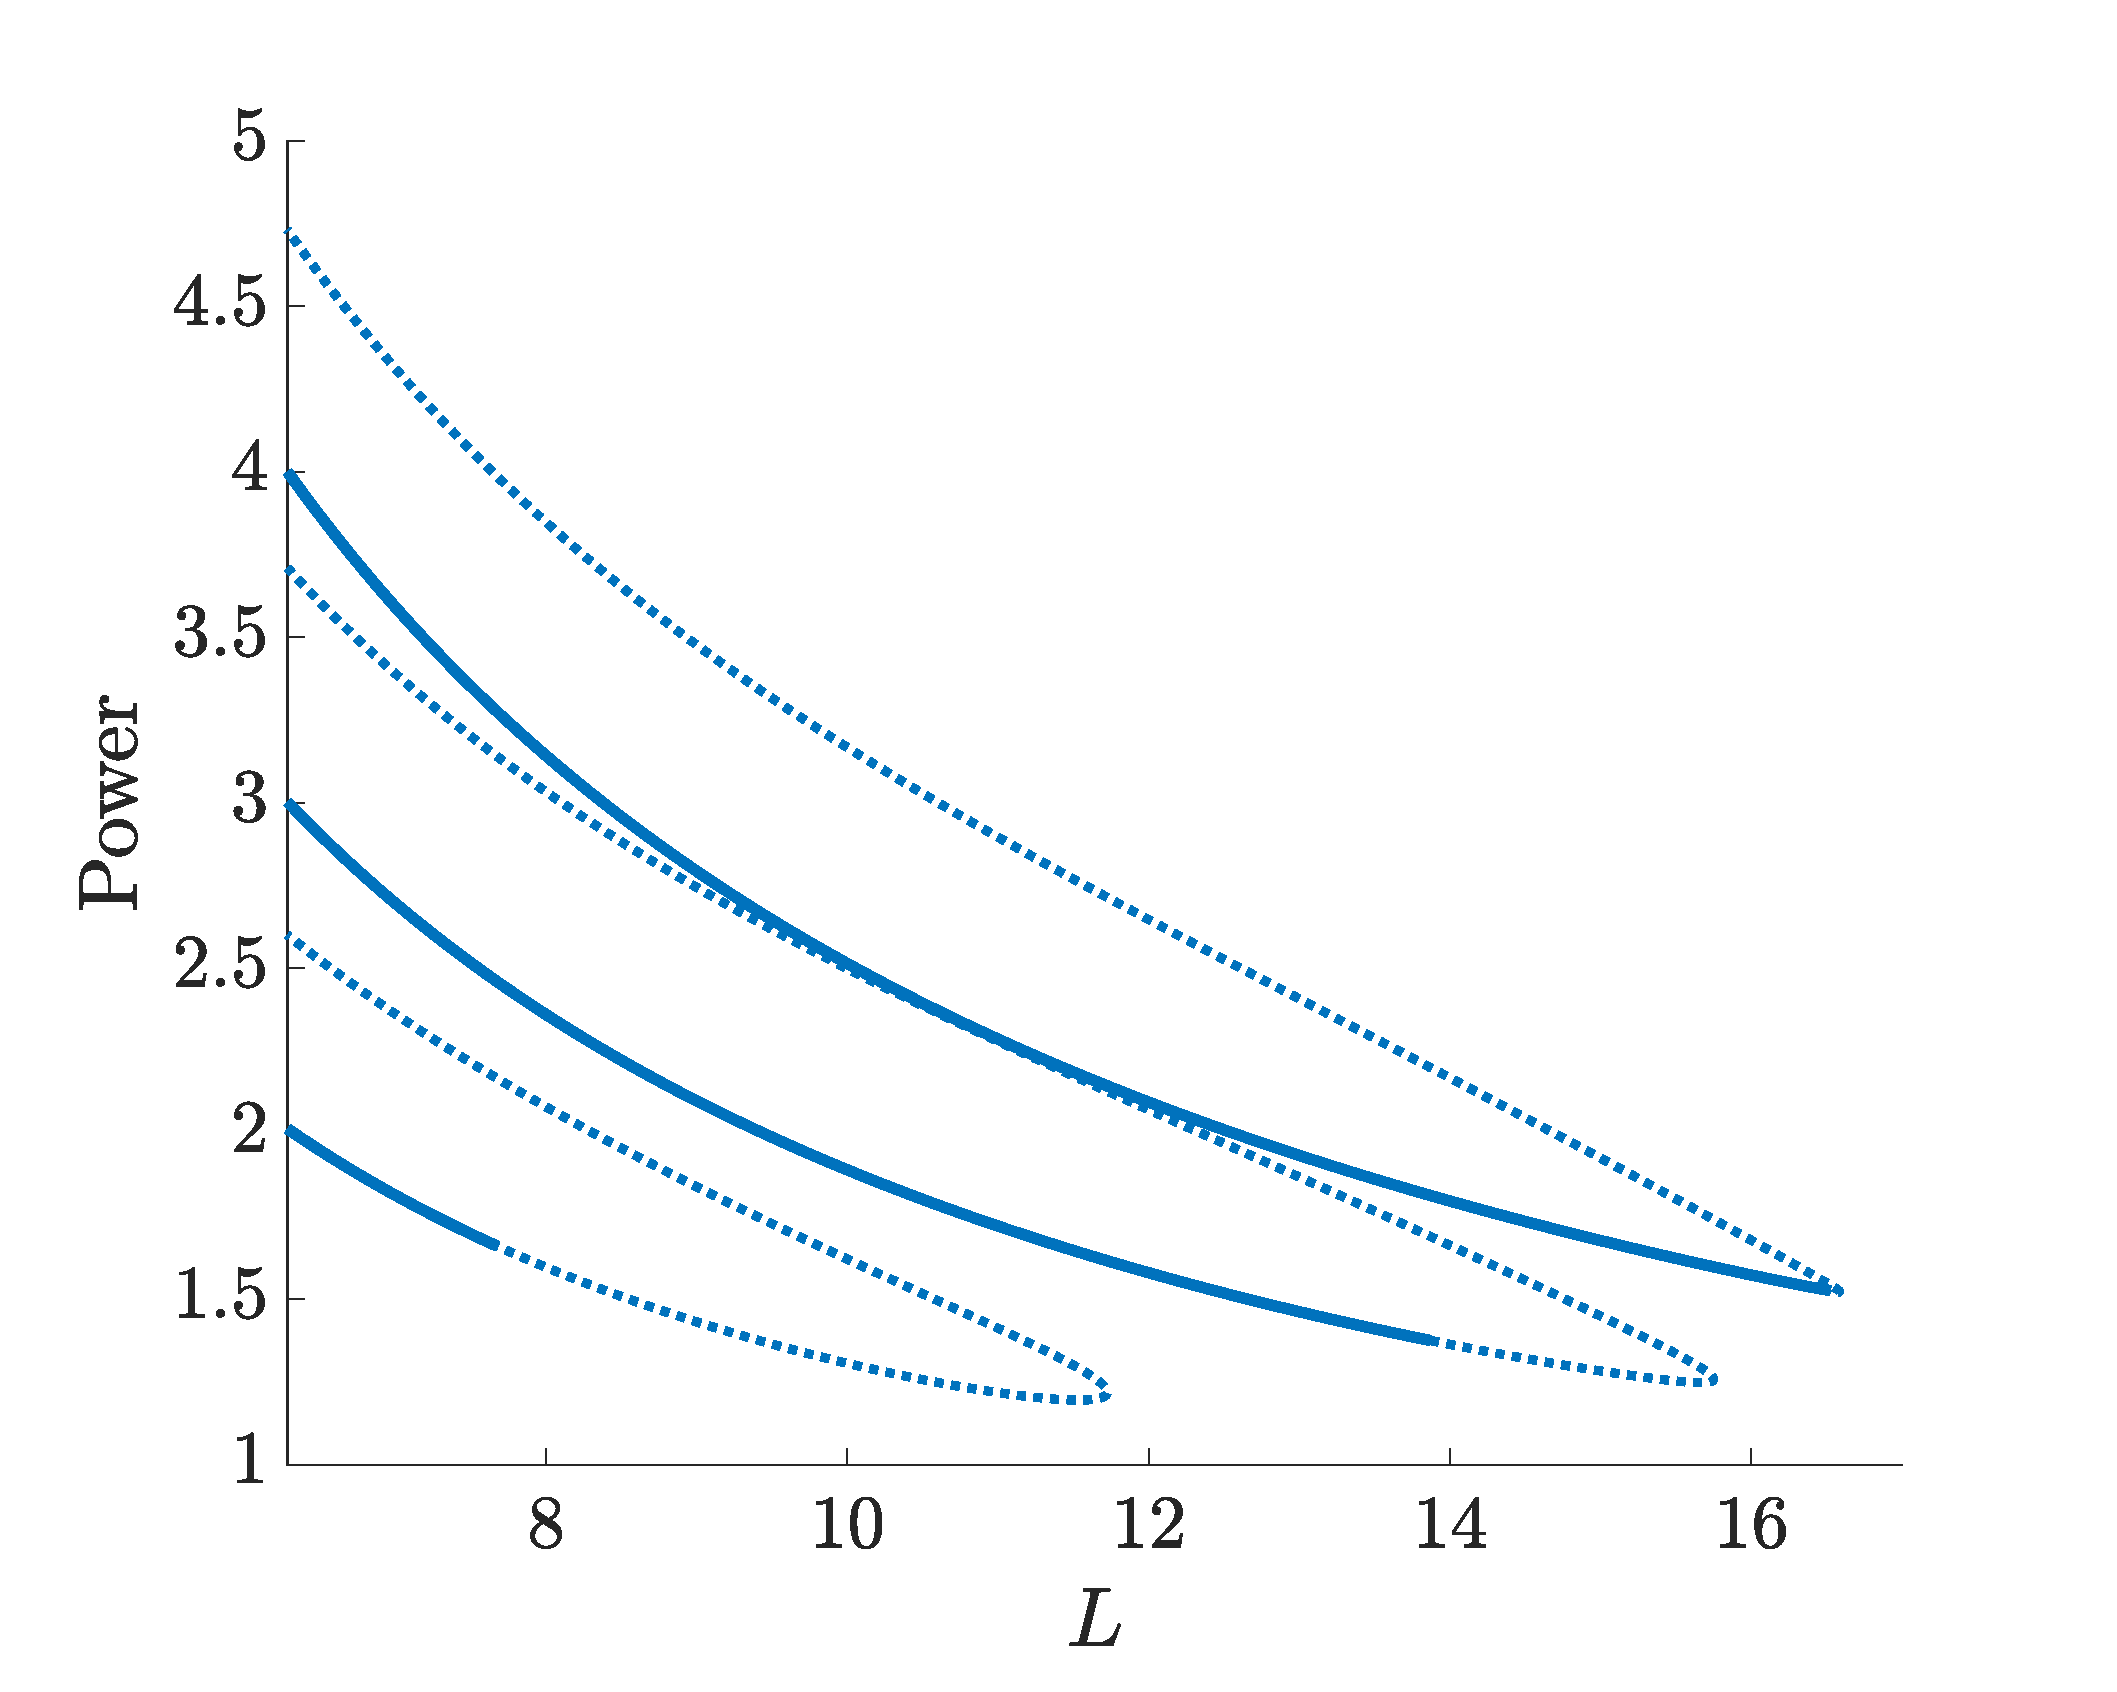
\includegraphics[width=8cm]{stat234contL.eps}
    \caption{Power vs. coupling period $L$ for solutions with approximate power of 2, and 4 at $L = 2\pi$. Solid lines correspond to solutions with Floquet spectrum contained in unit circle, dotted lines correspond to solution with some Floquet spectrum outside of unit circle. Diagram is only shown for $L\geq 2\pi$. Parameters $J_0 = 0.05$ and $C=0.25$.}
    \label{fig:statcontL}
\end{figure}

Finally, we note that, while we have only considered stationary solutions with period of 1, stationary solutions do exist for other positive integer periods. For example, if we start with a single-site initial condition with power $k/2$ for positive, odd integer $k$, we expect that we will obtain a stationary solution with period 2. (We have verified that this is the case for single-site initial conditions with power 3/2 and 5/2). While, in principle, this can be done for any integer period, it becomes computationally intractable for larger periods.

\subsection{Moving solutions}

Next, we look at the moving solutions. For a given lattice size $m$, we find that leftward moving solutions exist (\cref{fig:leftsol}) for all values of $C$ within an interval $[C_L(m), C_R(m)]$ (see top right and bottom left of \cref{fig:leftdiag}).
These are true coherent structures, in that the entire solution reproduces itself exactly after one period, shifted three sites to the left. (In the numerical simulation, where we are using periodic boundary conditions on the lattice, we can think of this as a ``circular shift''). Generically, these solutions have oscillatory tails (\cref{fig:leftsol}, top right), and the amplitude of these oscillations depends on the lattice size (\cref{fig:leftdiag}, top left). At a critical value $C^*$ of $C$ ($C^* = 0.4709$ for $J_0 = 0.05$ and $L=2\pi$), the tail oscillations vanish, leaving a localized traveling solution (\cref{fig:leftdiag}, bottom right). Most notably, the value of $C^*$ is independent of the lattice size $m$, although it does depend on both $L$ and $J_0$ (\cref{fig:Cstar}. The left moving solution appears to be stable when $C=C^*$ (see \cref{fig:movelong}, left); at minimum, it persists unchanged for at least 1000 periods. In addition, the solution appears to be stable for an interval in $C$ containing $C^*$ (not shown). Since the traveling solution is not a periodic orbit, we cannot use Floquet analysis to determine its spectral stability.wa
We note that while the parameter continuation in the bottom left of \cref{fig:leftdiag} continues past the turning points at $C_L(m)$ and $C_R(m)$, this merely represents growth of the tail oscillations, while the power of the central site remains essentially unchanged; since none of these solutions are stable, the continuation diagram is not shown past these turning points. 

Similar results are obtained for the right-moving solutions (\cref{fig:rightsol} and \cref{fig:rightdiag}). Once again, the tail oscillations vanish at a critical value $C^*$ of $C$ ($C^* = 0.5054$ for $J_0 = 0.05$ and $L=2\pi$), which is close, but not equal to, the value for the left-moving solution. The right-moving solution also appears to be stable at (and near) $C=C^*$ (see \cref{fig:movelong}, right). Unlike the left-moving solution, which is symmetric (\cref{fig:leftsol}, top left), the right-moving solution is asymmetric (\cref{fig:rightsol}, top left). For the initial condition of the right-moving solution, the power profile of the initial condition is skewed to the right. In addition, the power of the central site for the right-moving solution (approximately 0.6842) is significantly higher than that of the left-moving solution (approximately 0.3416).

\begin{figure}
    \centering
    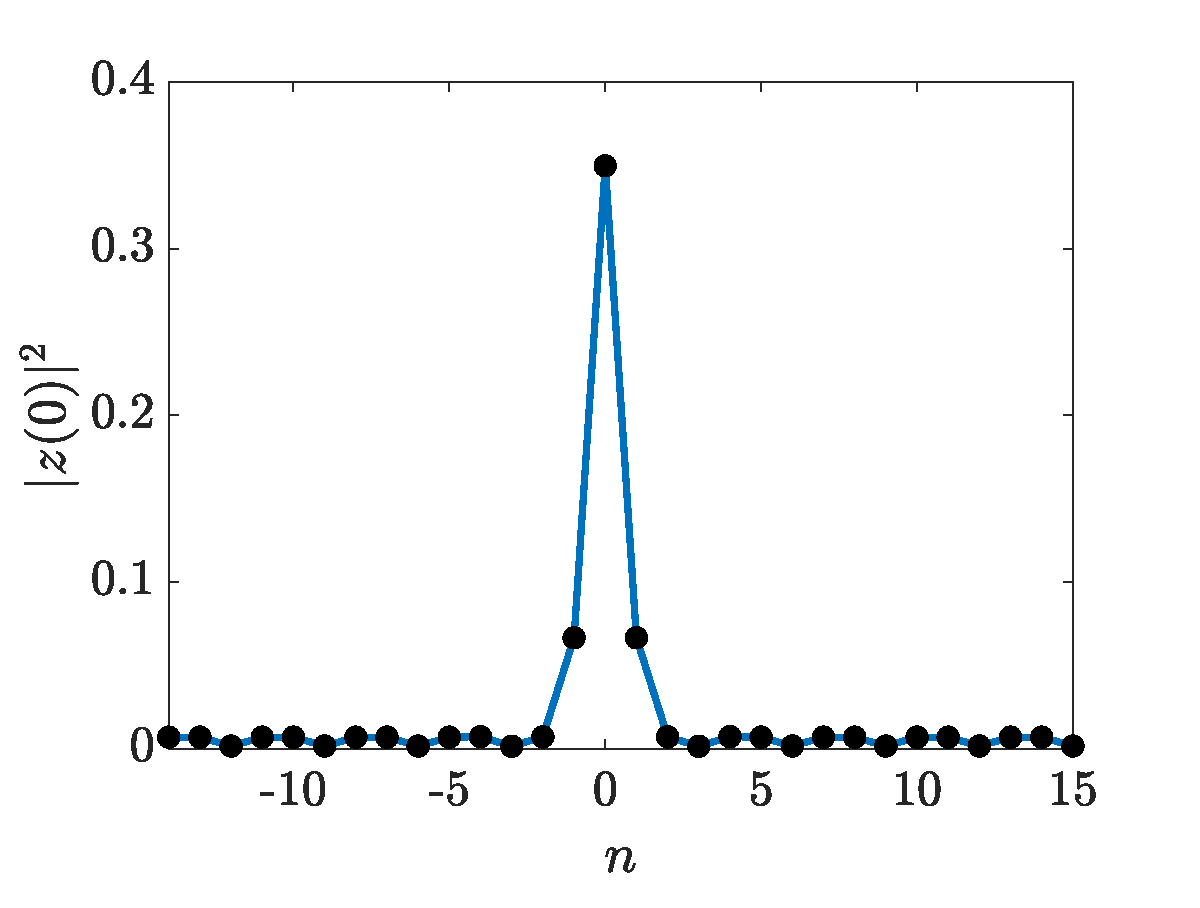
\includegraphics[width=9cm]{leftsol.eps}
    \caption{Initial power $|u_n(0)|^2$ (top left) and log of initial power (top right) for left-moving solution. Colormap showing power of solution evolved in $Z$ (bottom left), and power of central sites over one period (bottom right).}
    \label{fig:leftsol}
\end{figure}

\begin{figure}
    \centering
    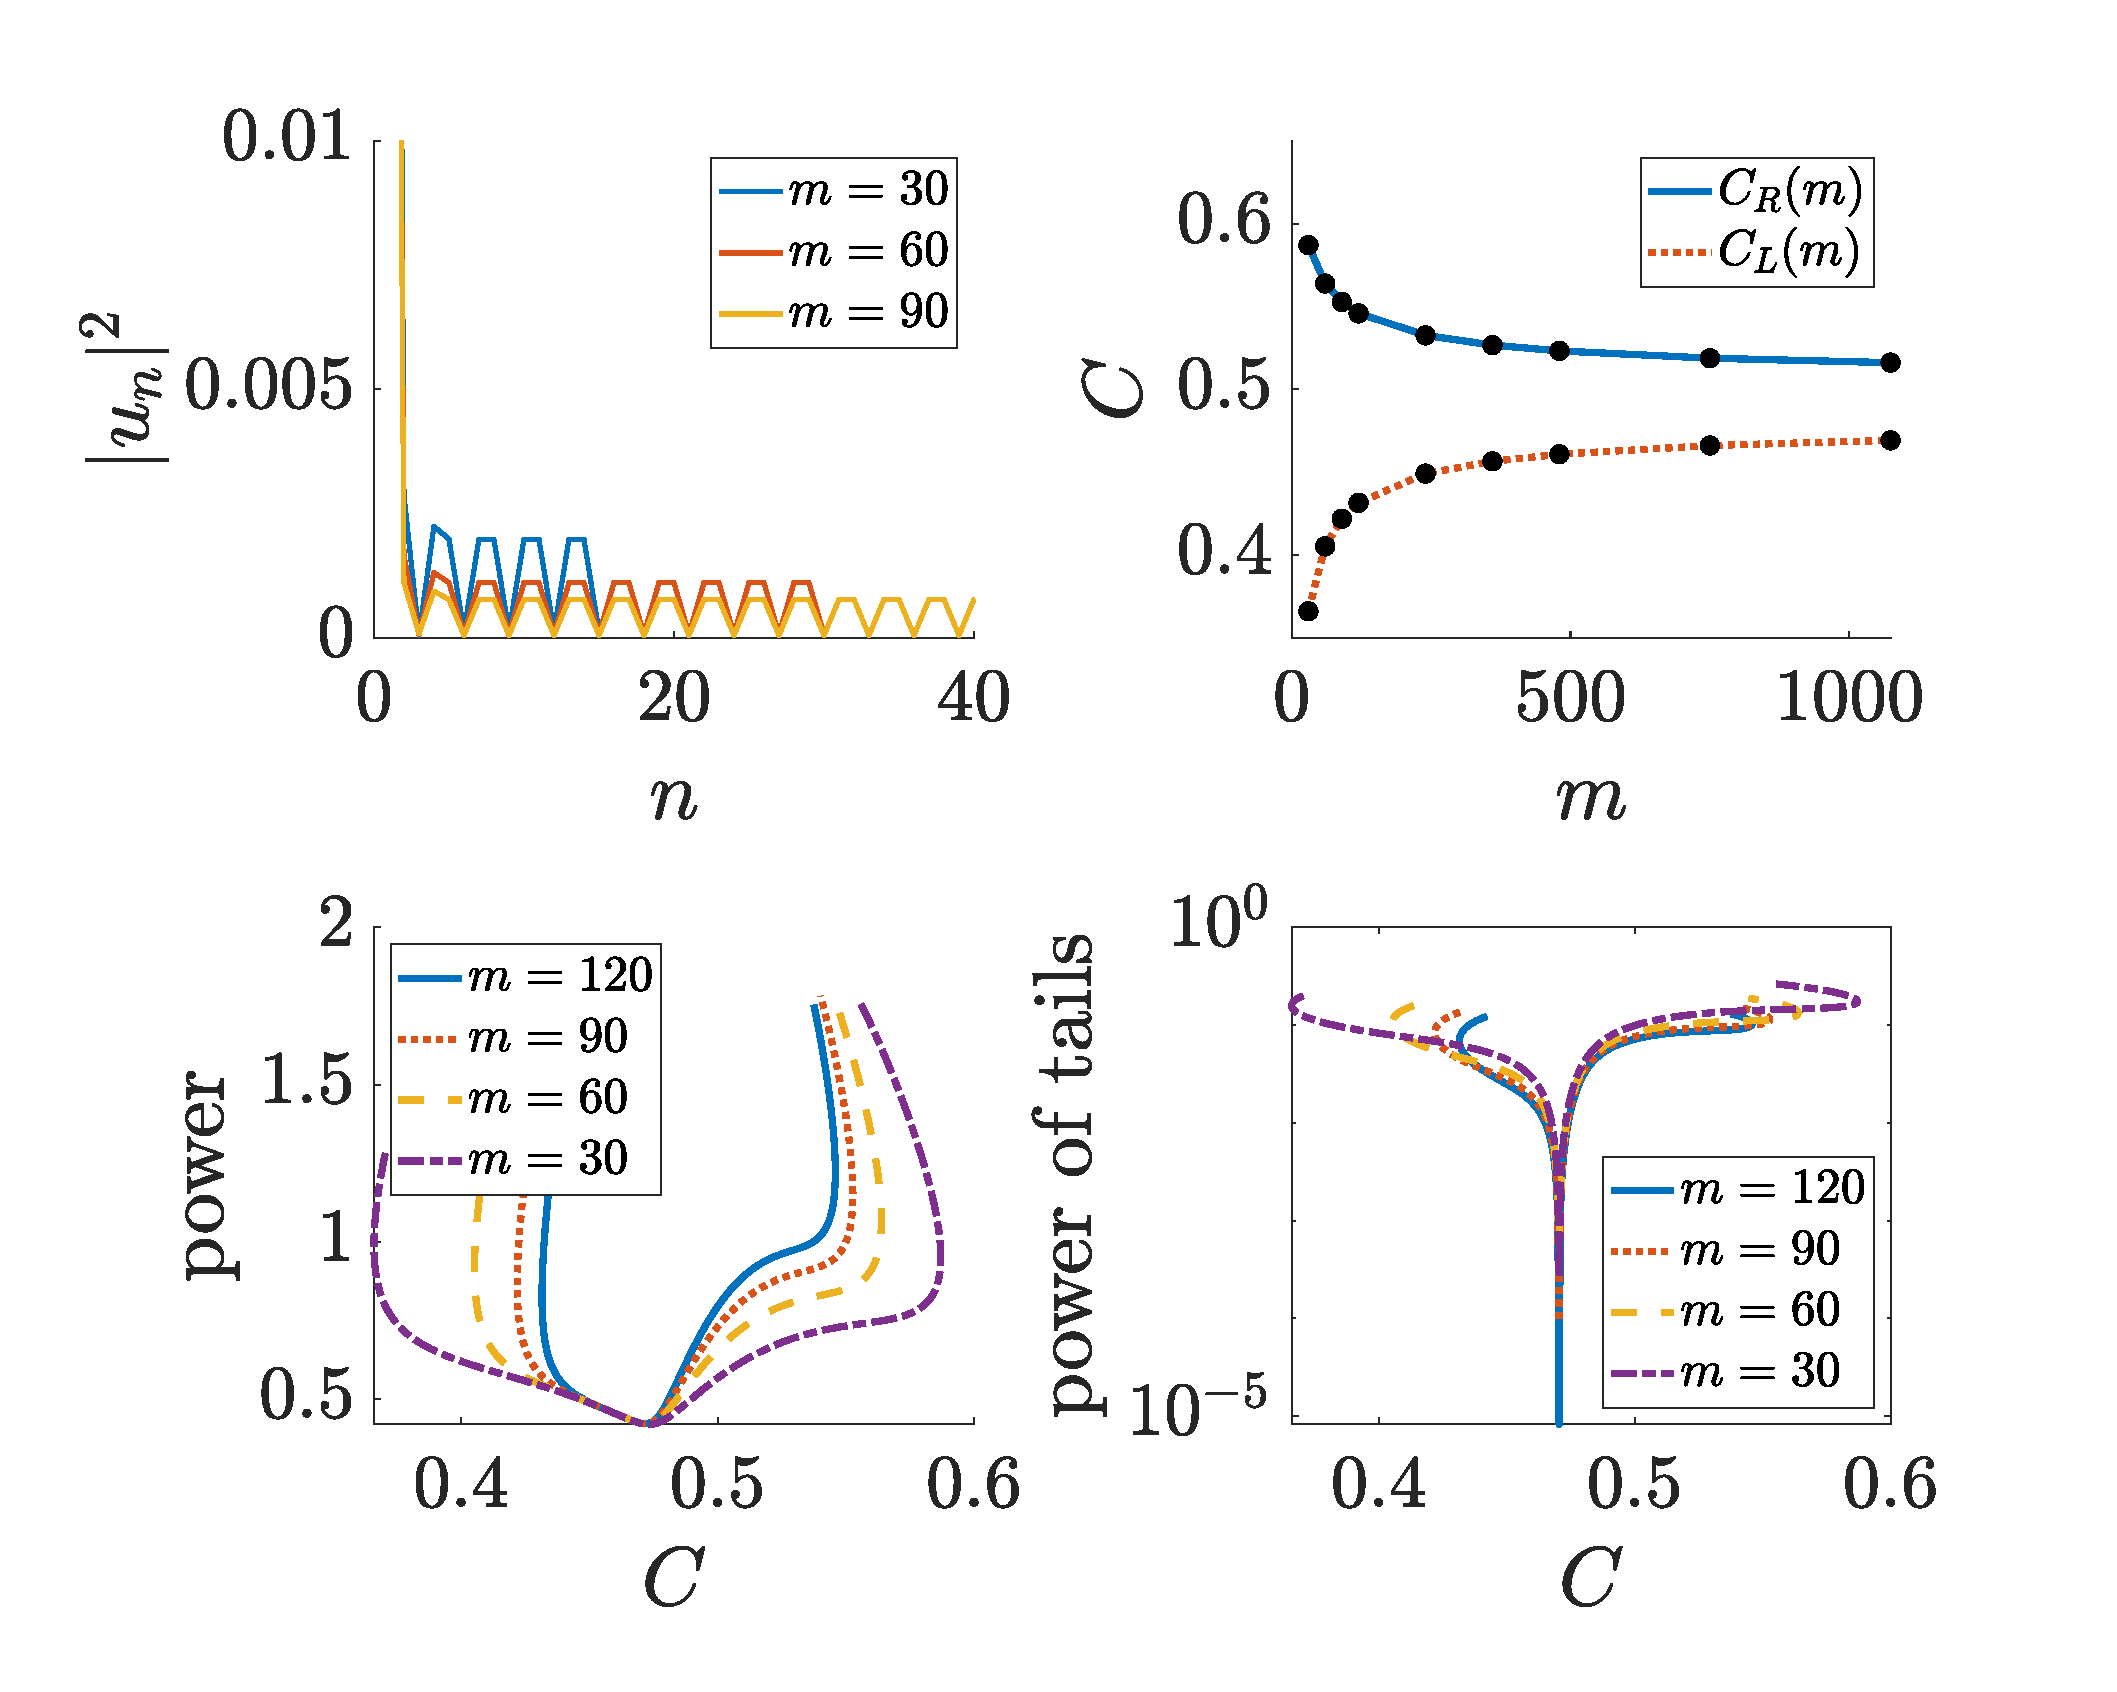
\includegraphics[width=9cm]{leftdiag.eps}
    \caption{Top left: plot of power of of tails of of left-moving solution for 3 values of the lattice size $m$. Top right: interval of existence $[C_L(m),C_R(m)]$ of left-moving solution. Bottom left: power of left-moving solution vs. $C$ for parameter continuation in $C$. Bottom right: maximum power of tails of left-moving solution vs. $C$. Minimum is at $C^* = 0.4709$ for all lattice sizes $m$.}
    \label{fig:leftdiag}
\end{figure}

\begin{figure}
    \centering
    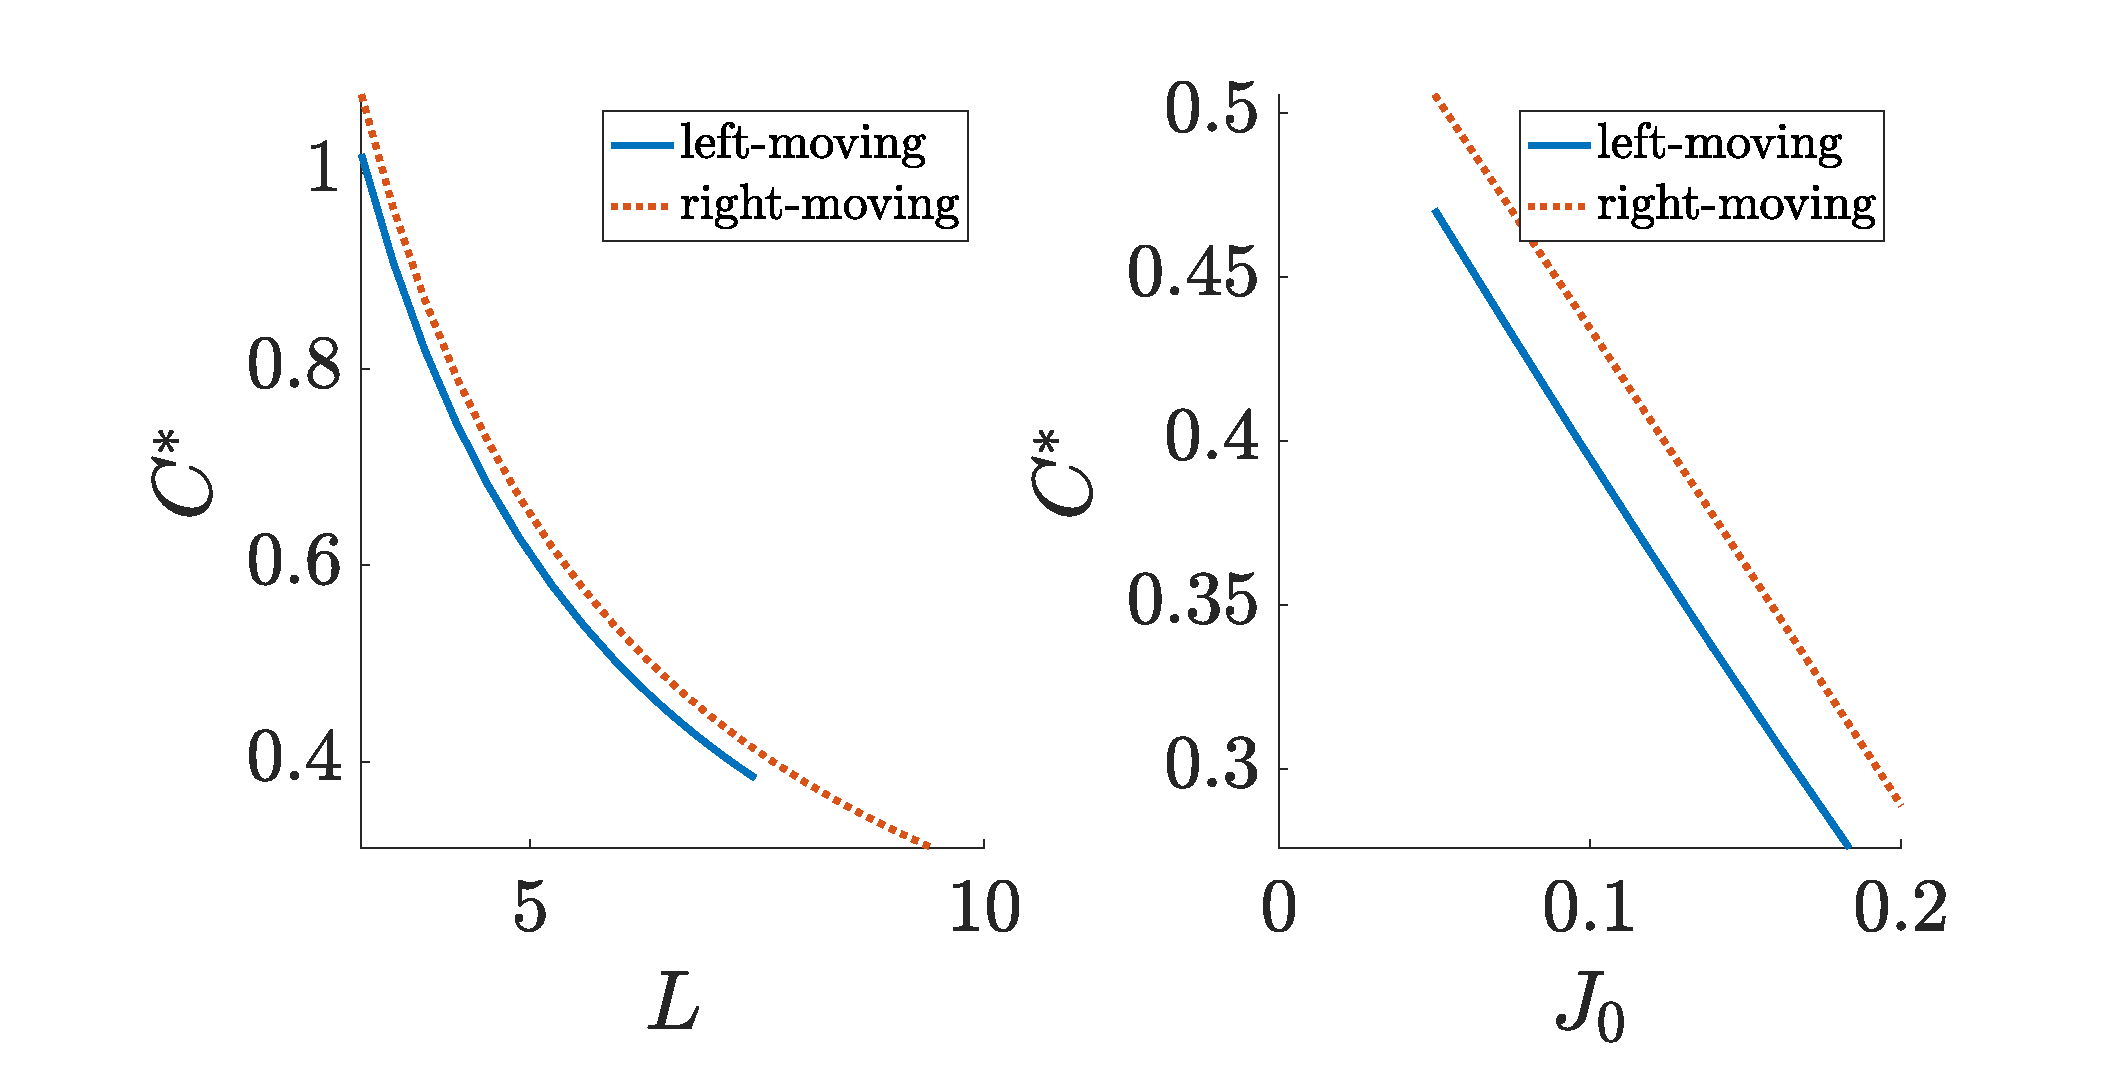
\includegraphics[width=9cm]{Cstar.eps}
    \caption{Plot of critical value $C^*$ of $C$ at which power of tails of left- and right-moving solution is a minimum vs. $L$ (left) and $J_0$ (right).}
    \label{fig:Cstar}
\end{figure}

\begin{figure}
    \centering
    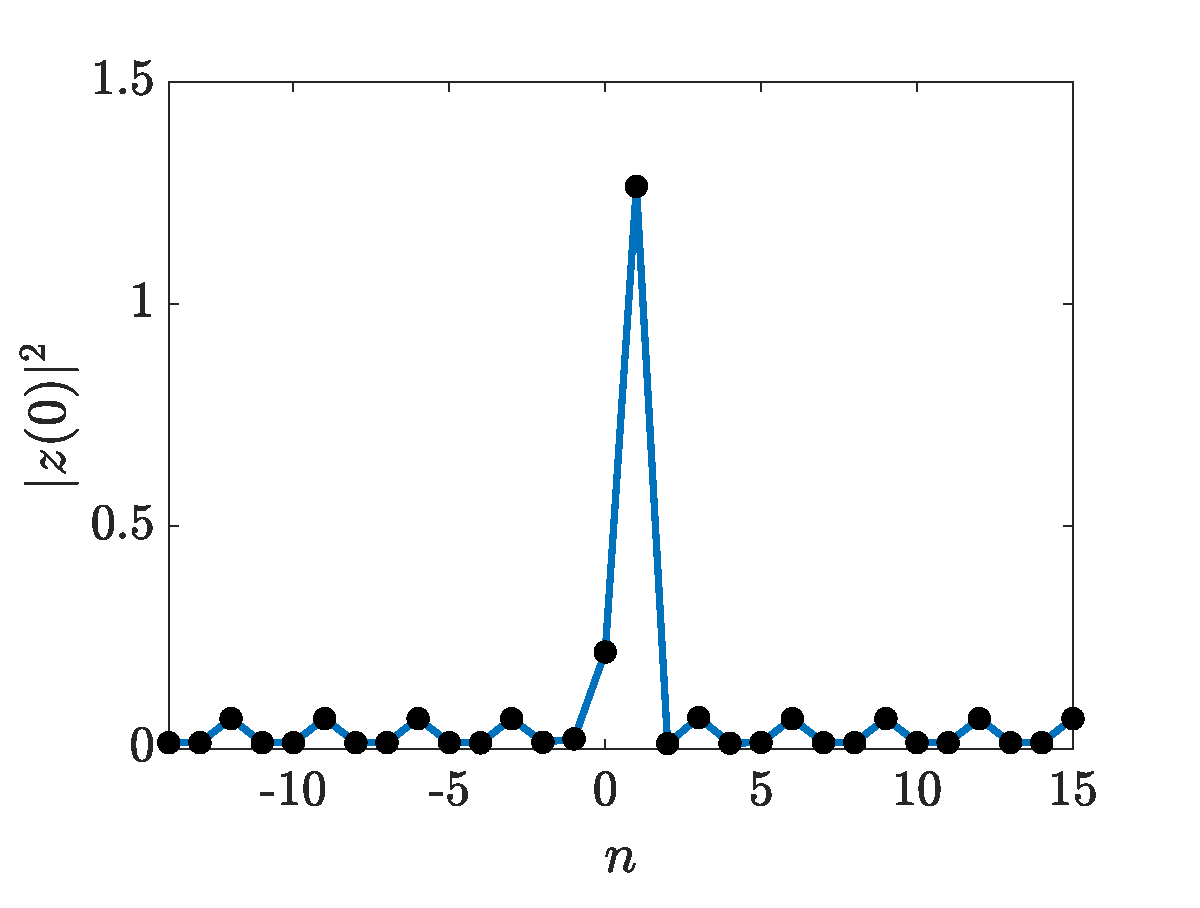
\includegraphics[width=9cm]{rightsol.eps}
    \caption{Initial power $|u_n(0)|^2$ (top left) and log of initial power (top right) for right moving solution. Colormap showing power of solution evolved in $Z$ (bottom left), and power of central sites over one period (bottom right).}
    \label{fig:rightsol}
\end{figure}

\begin{figure}
    \centering
    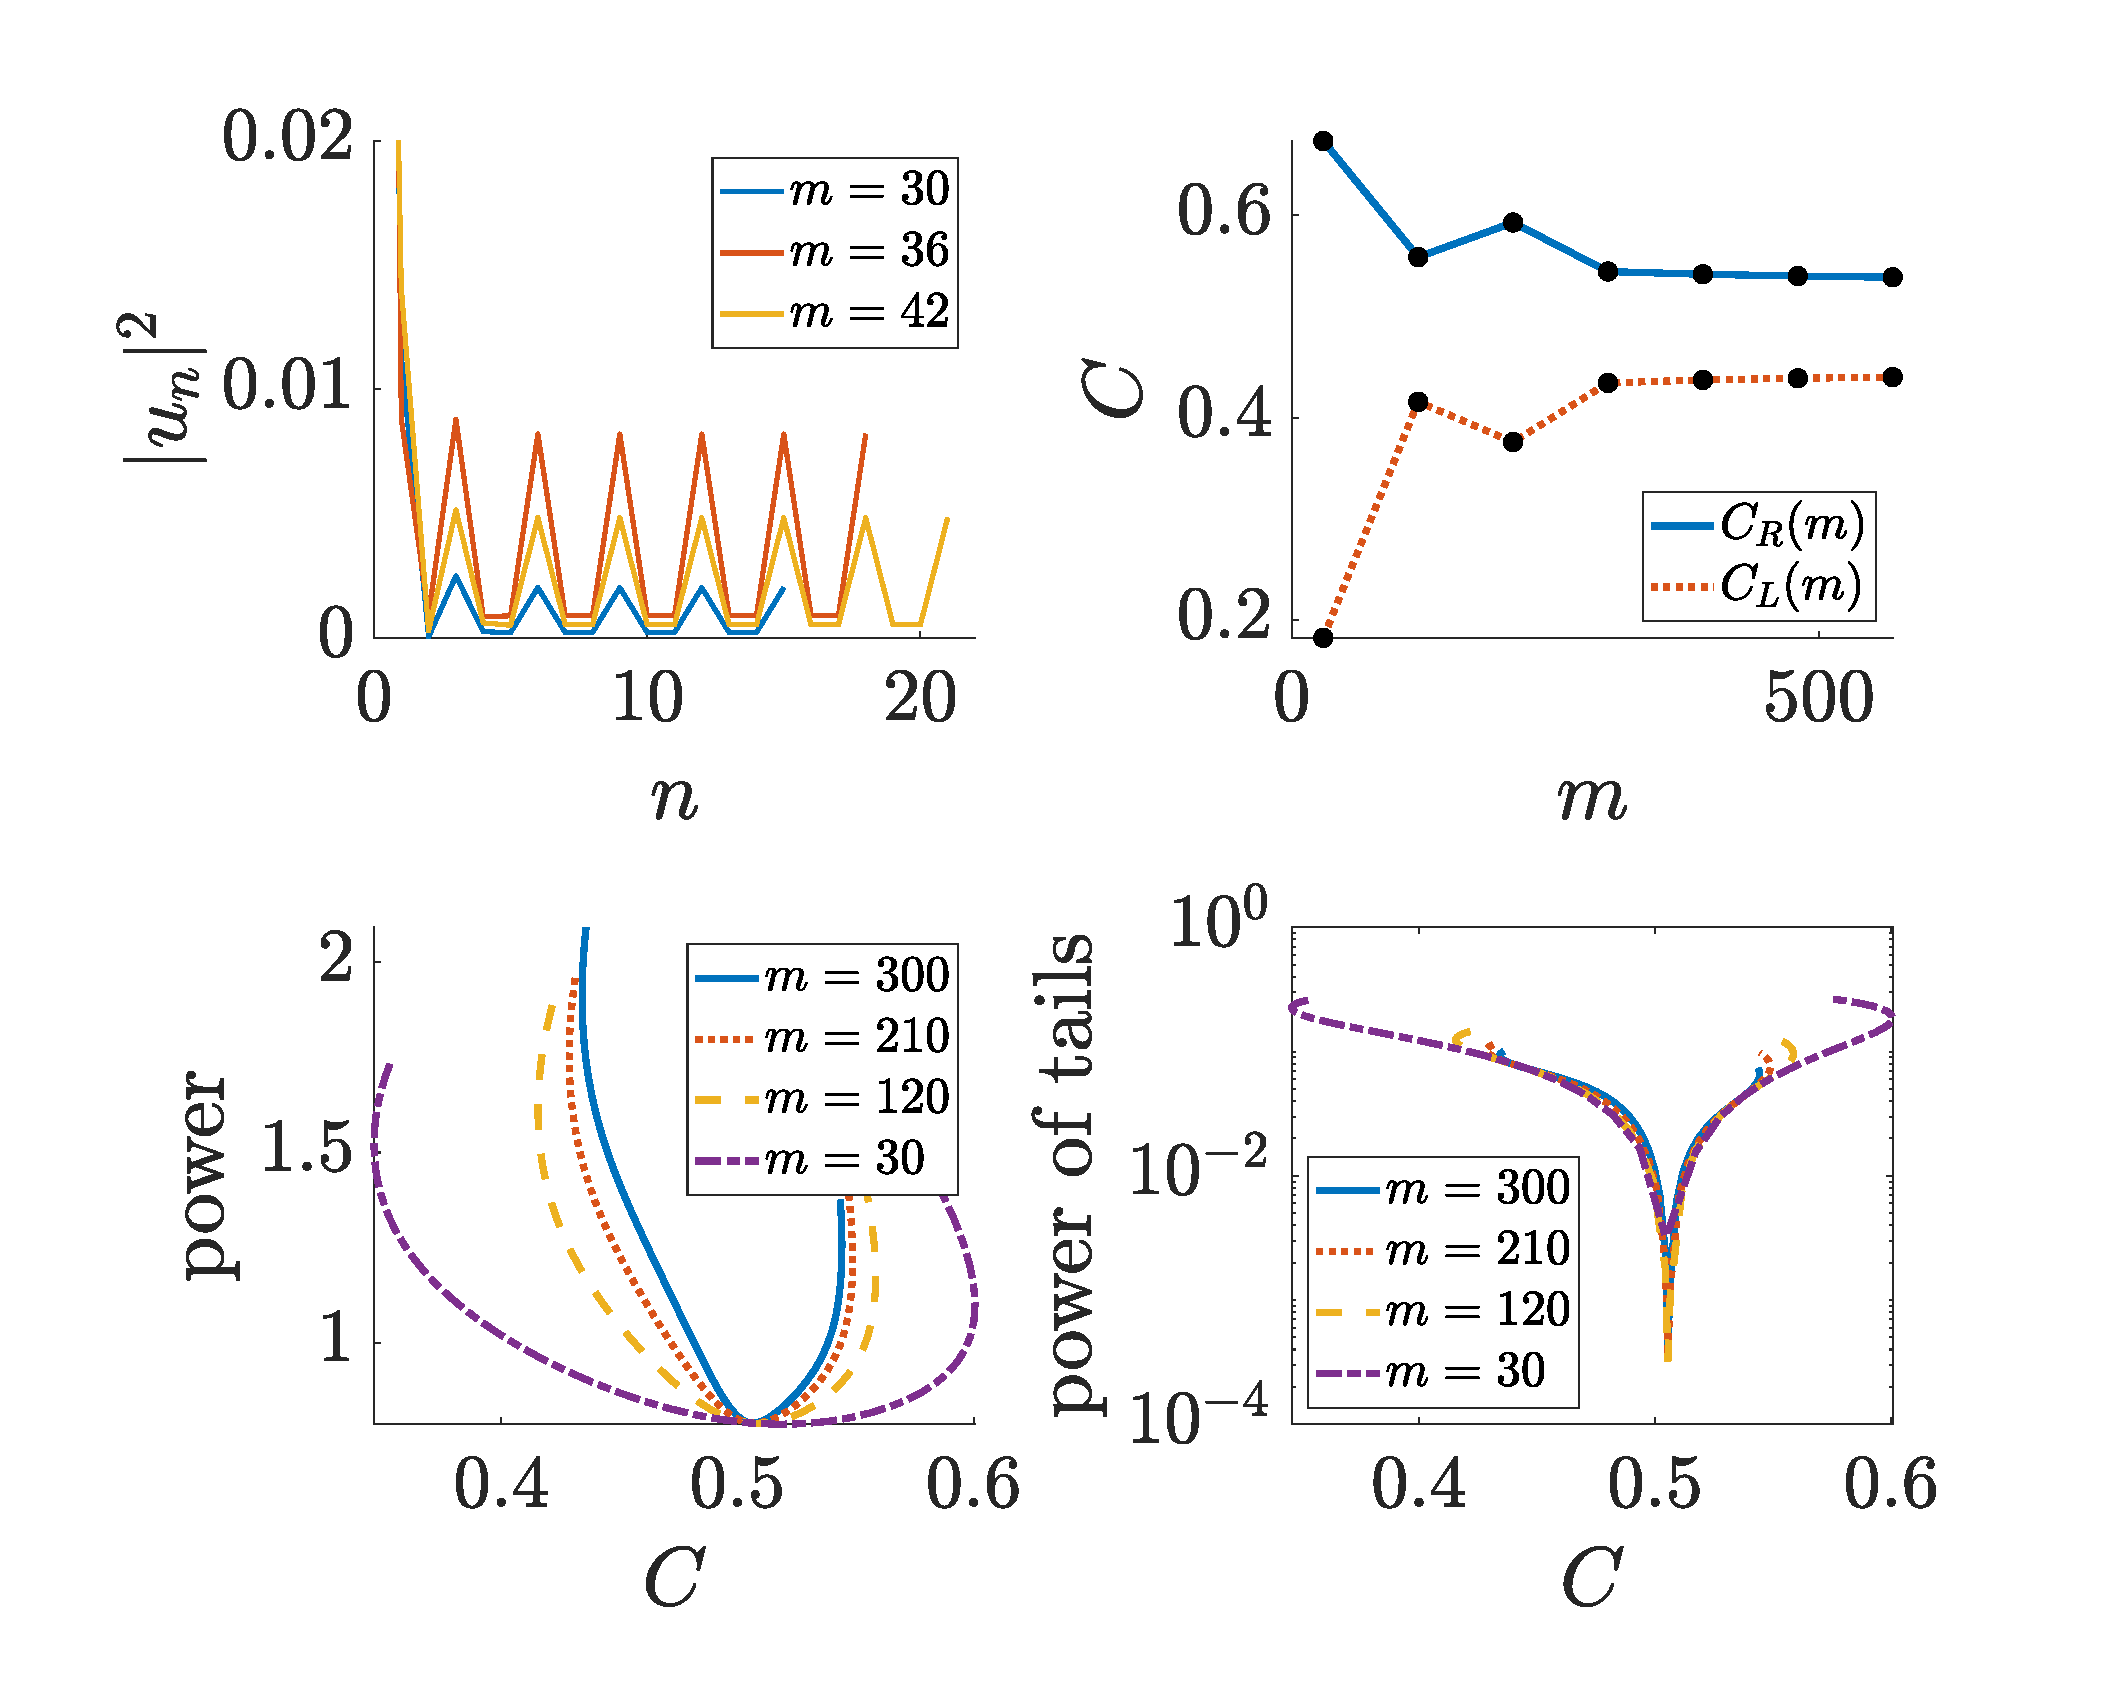
\includegraphics[width=9cm]{rightdiag.eps}
    \caption{Top left: plot of power of of tails of of right-moving solution for 3 values of the lattice size $m$. Top right: interval of existence $[C_L(m),C_R(m)]$ of right-moving solution. Bottom left: power of right-moving solution vs. $C$ for parameter continuation in $C$. Bottom right: maximum power of tails of right-moving solution vs. $C$. Minimum is at $C^* = 0.5054$ for all lattice sizes $m$.}
    \label{fig:rightdiag}
\end{figure}

\begin{figure}
    \centering
    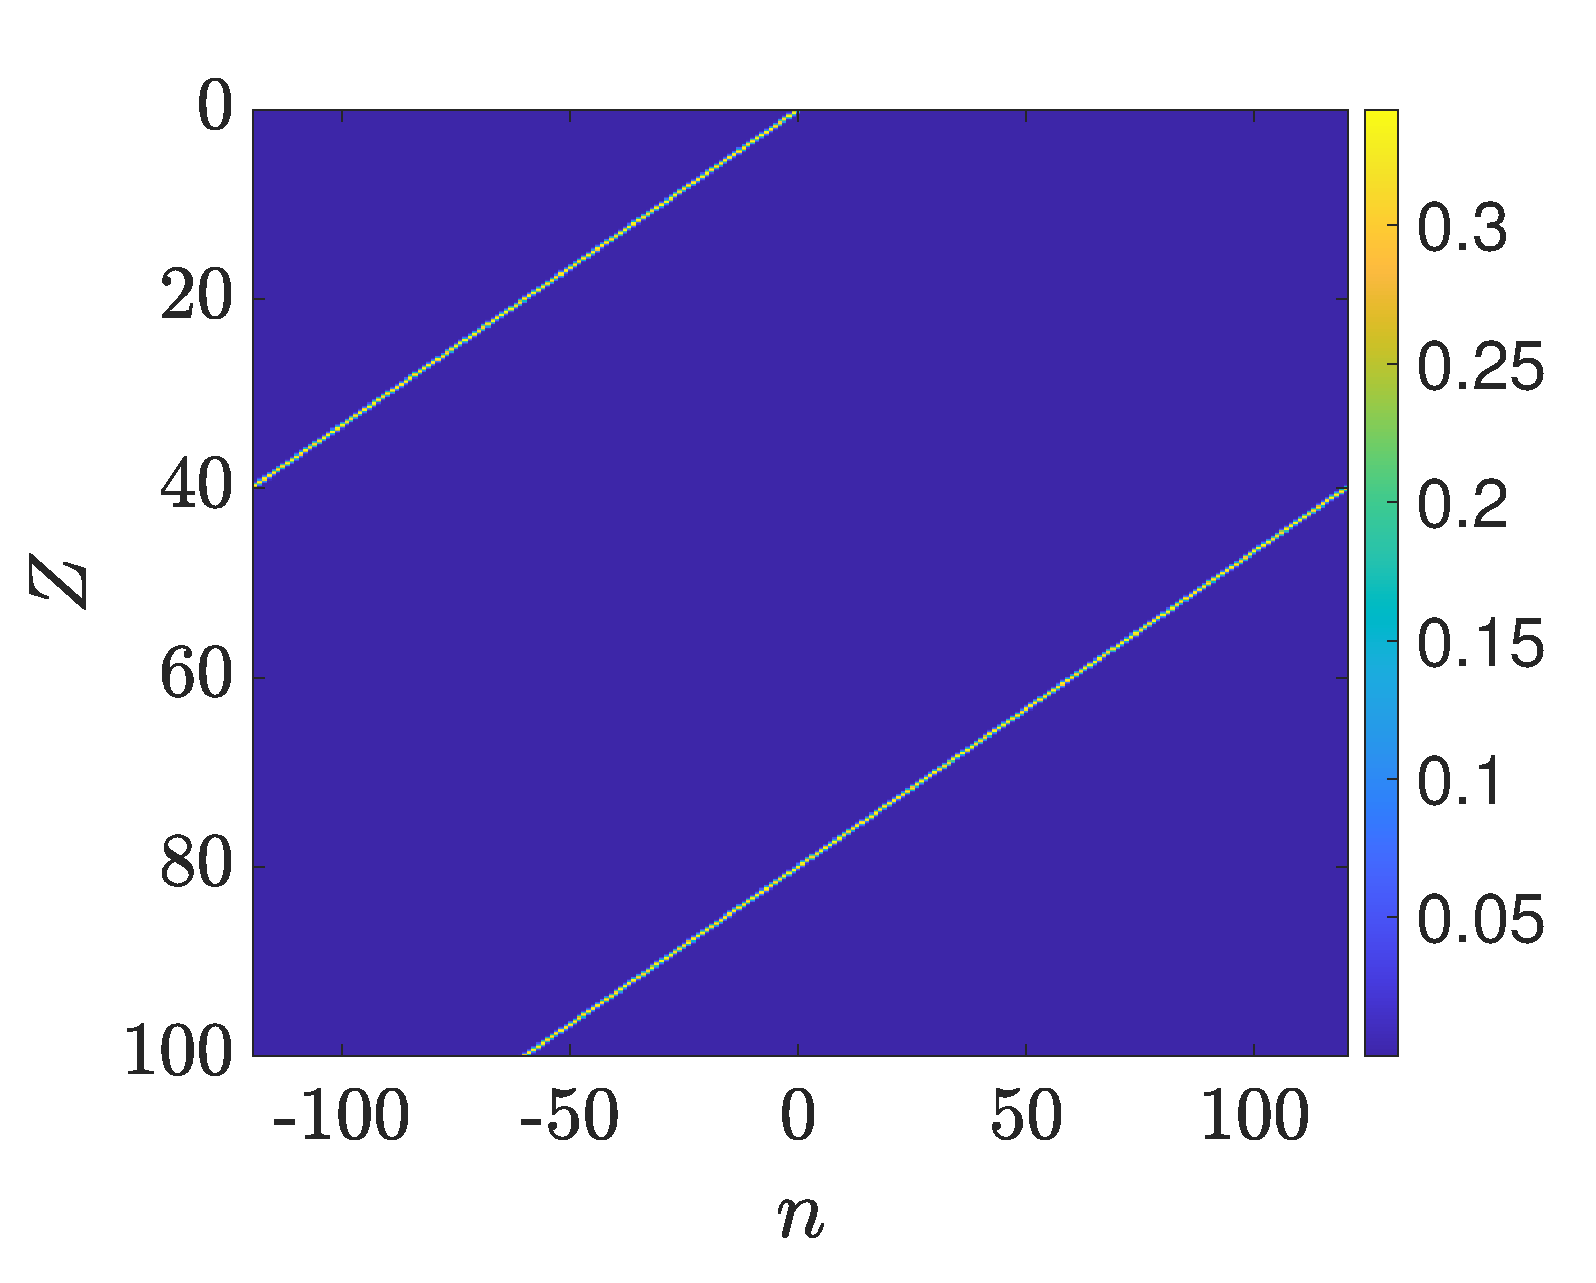
\includegraphics[width=3.90cm]{leftlong.eps}
    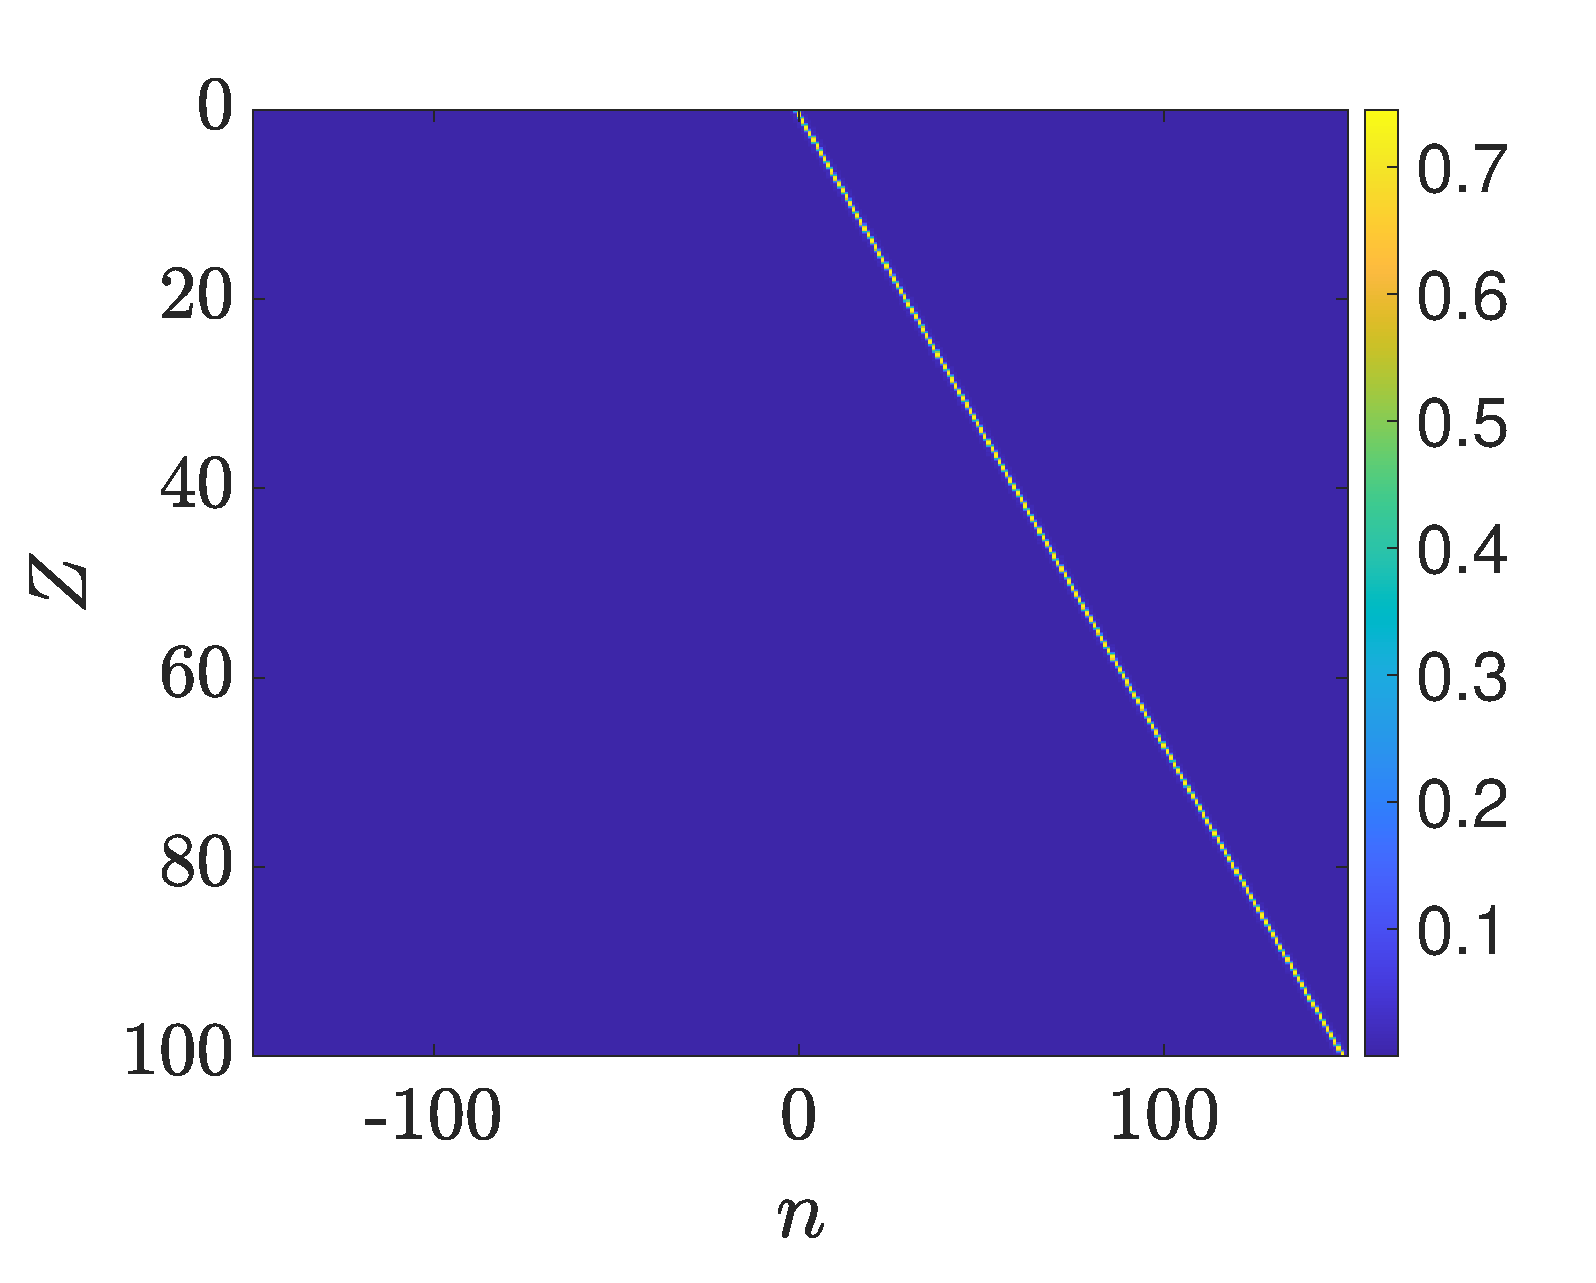
\includegraphics[width=3.90cm]{rightlong.eps}
    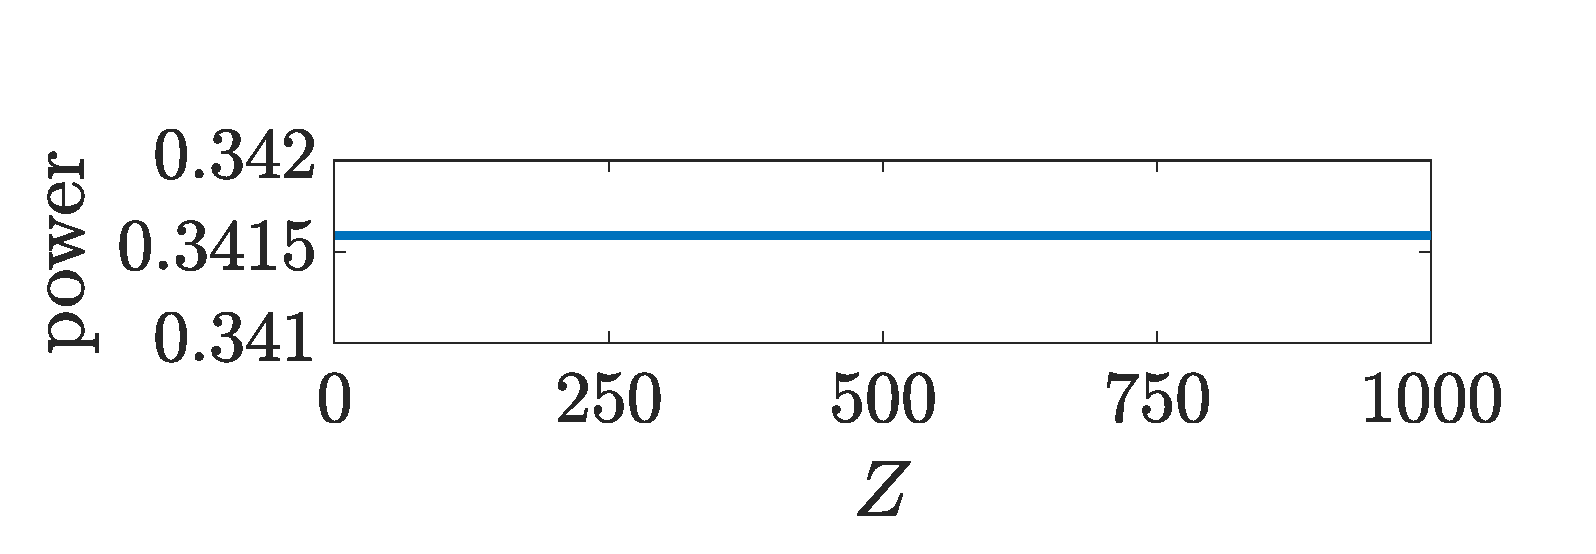
\includegraphics[width=3.90cm]{leftperiods.eps}
    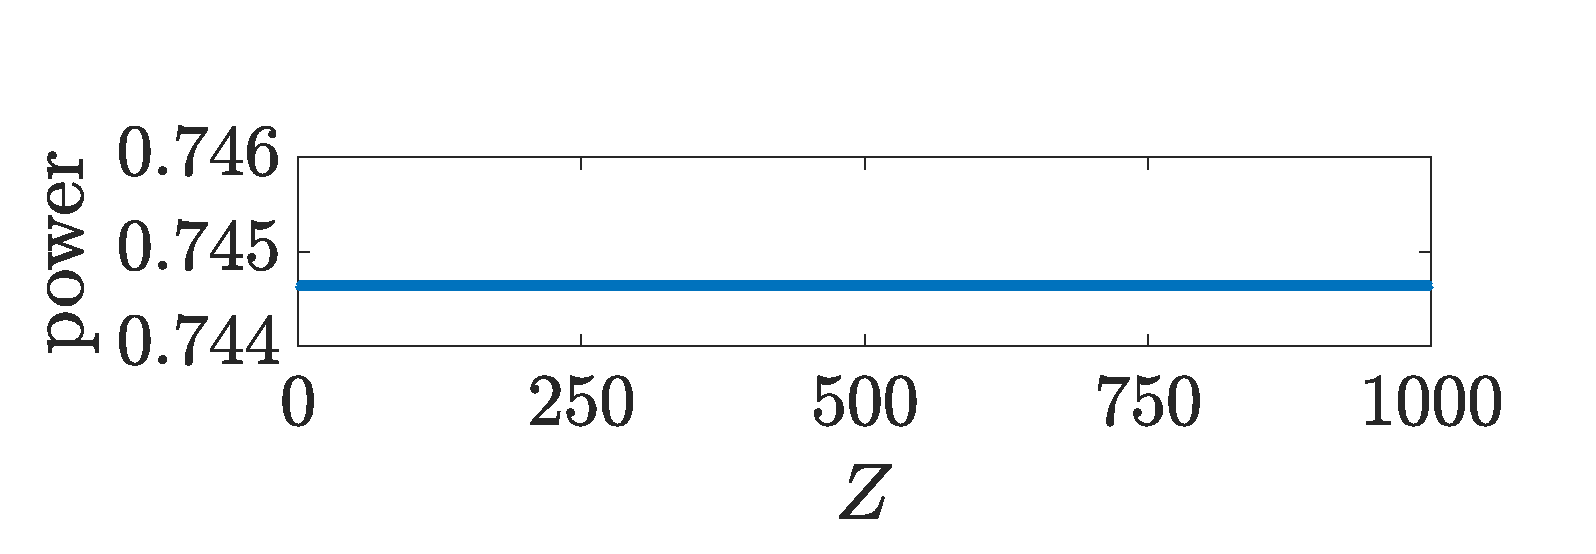
\includegraphics[width=3.90cm]{rightperiods.eps}
    \caption{Top: colormap of long term evolution in $Z$ of left-moving solution (left, $C=0.4703$, $m=240$) and right-moving solution (right, $C=0.5054$, $m=300$) for $C=C^*$. Bottom: power of site with peak intensity of moving solution over 1000 periods.}
    \label{fig:movelong}
\end{figure}

\subsection{Collisions}

Finally, we briefly explore what occurs when a left-moving and a right-moving solution collide \cref{fig:collision1}. For an initial condition, we splice together well-separated copies of the left-moving and right-moving solutions. To avoid combining the tail oscillations of the two solutions, we choose $C=C^*$ for the left-moving solution, so that its tail oscillations are suppressed. We see that both solutions emerge from the first collision, but both solutions lose power as intensity radiates to the left. Power is lost with each subsequent collision (\cref{fig:collision1}, bottom).

\begin{figure}
    \centering
    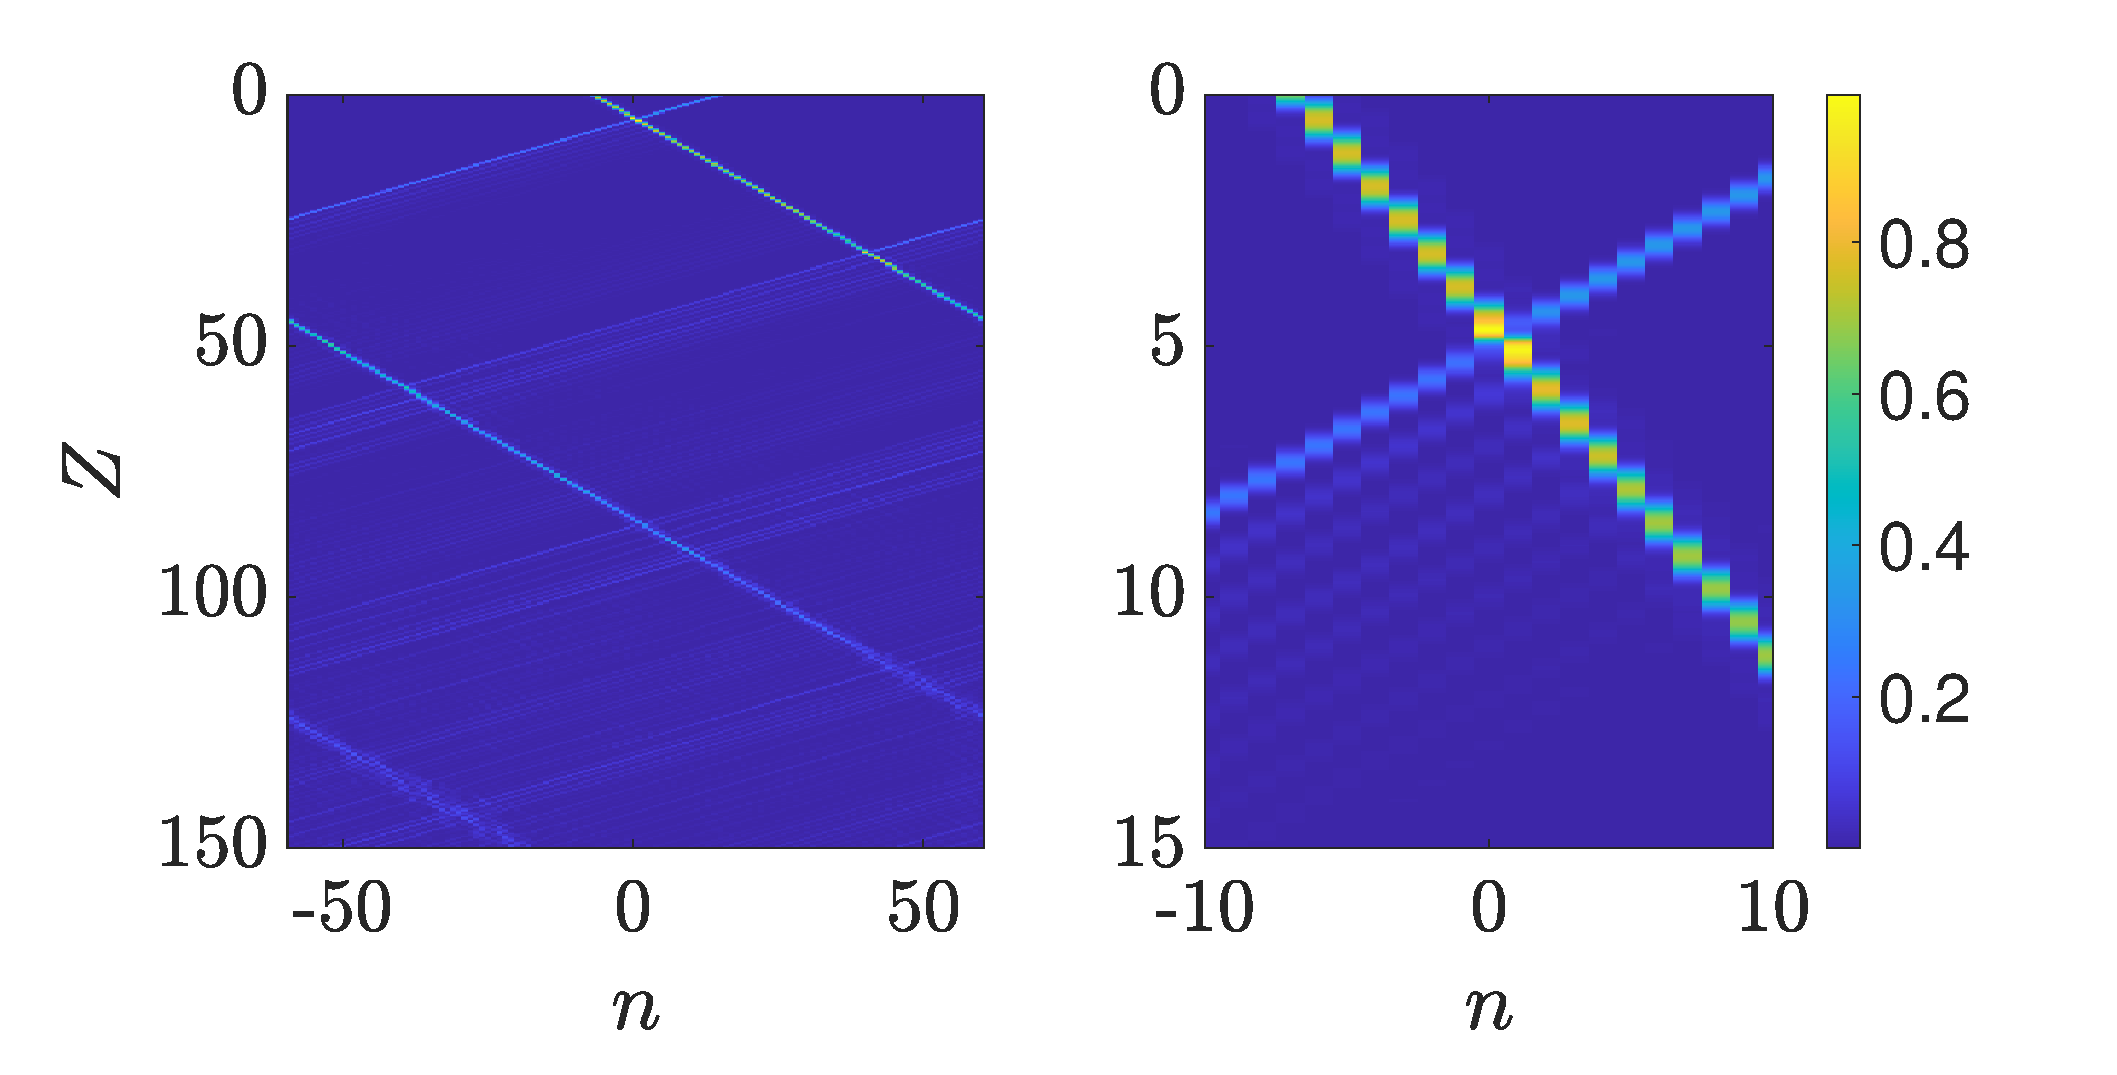
\includegraphics[width=9cm]{images/collision1.eps}
    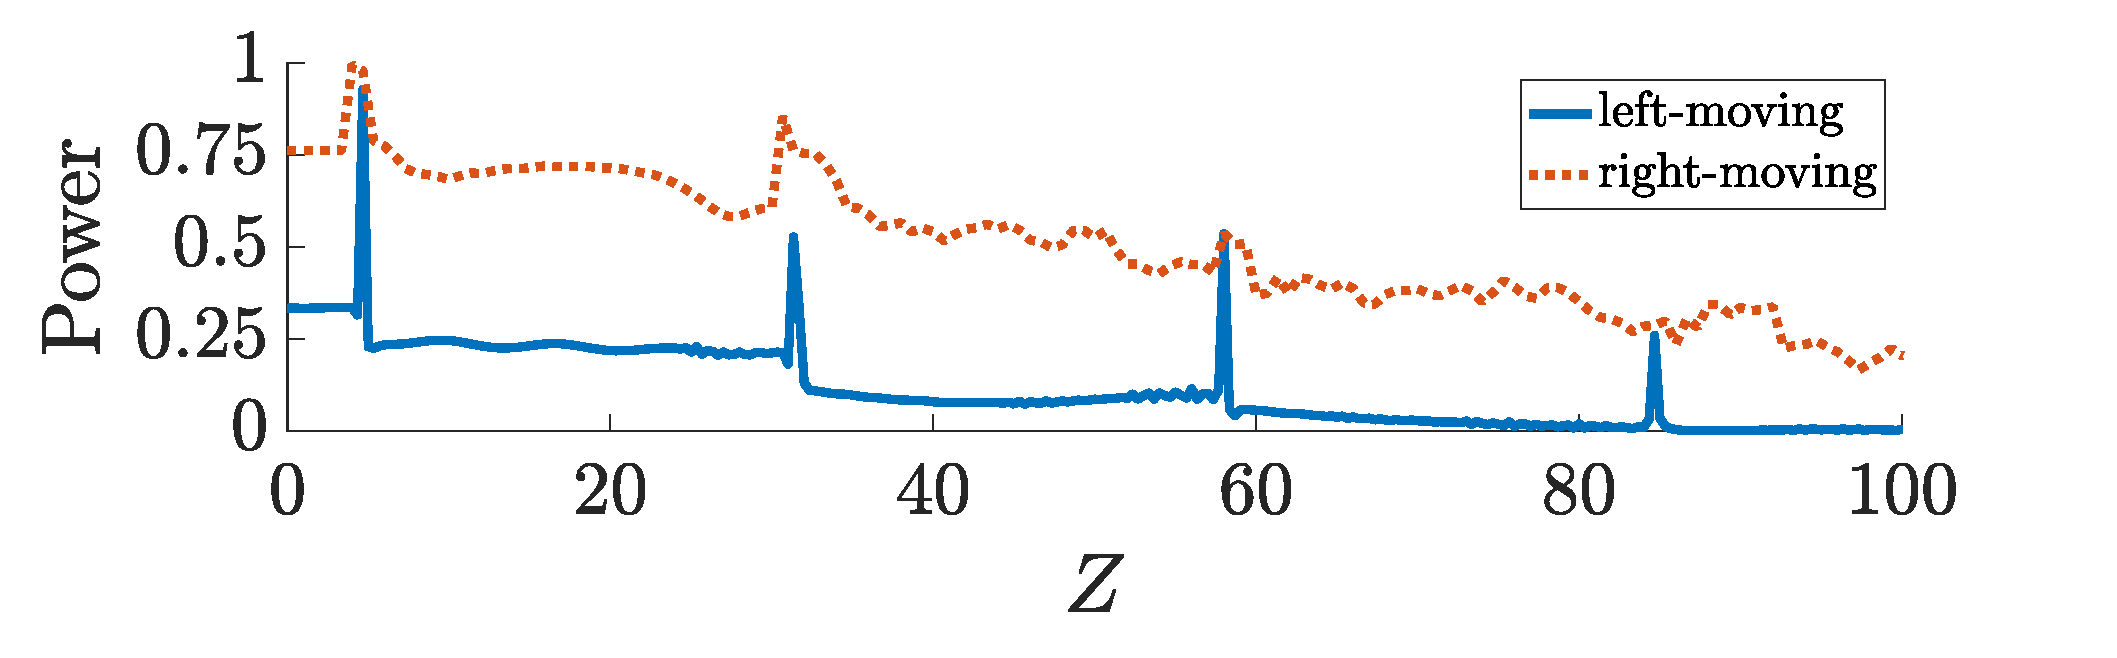
\includegraphics[width=9cm]{images/collision1power.eps}
    \caption{Top: Colormap of evolution in $Z$ of collision between left-moving and right-moving solution. Right panel is a zoomed-in view of the first collision. Bottom: power of site with peak intensity of left- and right-moving solutions.
    $m=120$, $C=0.4703$.}
    \label{fig:collision1}
\end{figure}


\bibliographystyle{amsplain}
\bibliography{main.bib}


\end{document}